\documentclass[conference,a4paper]{IEEEtran}

\usepackage[T1]{fontenc}
\setlength{\emergencystretch}{2em}
\usepackage[english]{babel}
\usepackage{booktabs}
\usepackage{stfloats}
\usepackage[hidelinks]{hyperref}
\usepackage{pgfplots}
\pgfplotsset{compat=1.18}
\usetikzlibrary{arrows.meta,decorations.pathreplacing}
% Okabe-Ito palette, readable with colour vision deficiencies
\definecolor{okVermillion}{HTML}{D55E00}
\definecolor{okSky}{HTML}{56B4E9}
\definecolor{okOrange}{HTML}{E69F00}
\definecolor{okGreen}{HTML}{009E73}
\definecolor{okBlue}{HTML}{0072B2}
\DeclareUrlCommand\param{\urlstyle{tt}\def\UrlBreaks{\do\-\do\=}}

\title{Measuring the Overhead of Trust Mechanisms\\in the X-Road Data Exchange Layer}
\author{\IEEEauthorblockN{Ruslan Nechshadimov}}

\newcommand{\newtext}[1]{{\color{blue}#1}}
\newcommand{\newred}[1]{{\color{red}#1}}
\newcommand{\newgreen}[1]{{\color{green!50!black}#1}}
\newcommand{\newviolet}[1]{{\color{violet}#1}}

\raggedbottom
\begin{document}
\maketitle
\thispagestyle{plain}
\pagestyle{plain}

\begin{abstract}
\newtext{X-Road secures data exchange between organisations with signatures, certificate status
checks, time-stamps and a message log, and proposed changes to these mechanisms, such as post-quantum
signatures, need a baseline for what they cost now. This study measures the per-message overhead of
the trust mechanisms of X-Road 7.8.3 on one and on three laptops\newtext{, on a faster development laptop} and with a round-trip time added
between the Security Servers, using configuration changes, per-stage timings and packet captures. With one client the X-Road path
adds about 28\,ms to a 10\,KB exchange. Signing and verification take only a few milliseconds of it; most
is \newtext{residual processing} of the Security Server, while logging the body takes almost half of a 1\,MB
exchange and synchronous time-stamping adds about 90\,ms. With an added round-trip time, opening a
new connection for every message, the default, has the largest effect: a message waits for about
five round trips at 10\,KB and ten at 1\,MB, against two with reused connections.} \newtext{An
estimate for post-quantum message signatures, from a benchmark on the platform of X-Road and from
messages padded to their size, changes the computation by about a millisecond \newtext{with the
lattice schemes and by up to 9\,ms with composites with RSA or SLH-DSA in the certification
authority}, while the size adds up
to two round trips with ML-DSA and five with SLH-DSA in the certification authority, only on new
connections and mostly through the signatures of the infrastructure. Under the evaluated conditions,
the latency added over distance is thus governed by new connections and the TCP window rather than by
the cryptography.}
\end{abstract}

\section{Introduction}

When one organisation acts on data received from another, it depends on something it did not
produce and cannot check by itself. Trust is the name for that dependence. In organisational
research it is defined as the willingness of a party to be vulnerable to the
actions of another party, based on the expectation that the other will perform an action important
to the trustor, without being able to monitor or control it~\cite{mayer1995}. In computing the same
idea is phrased as a belief in the competence of an entity to act dependably, securely and reliably
within a specified context~\cite{grandison2000}. In security engineering a \emph{trusted} component
is distinguished from a \emph{trustworthy} one: the first is a component whose failure can break the
security policy, the second one that will not fail~\cite{anderson2020}. A well-designed system therefore
tries to need as little trust as possible, and to place the rest in a few components that are named
explicitly and protected accordingly.

X-Road, the data exchange layer, is built on this principle. Its member organisations do not have to trust each other's
systems directly. Their trust rests on a root of trust, a point that is accepted as trusted
axiomatically~\cite{bakhtina2023sac}. In X-Road this root is centralised: it is formed by the
certification authorities that vouch for the members' keys~\cite{bakhtina2023sac}, together with the
Central Server, which publishes who the members are and which authorities to trust, and the
time-stamping authority~\cite{xroadarcss}. Every message then carries evidence that can be checked
against this root. It is signed by the sender's Security Server and verified by the receiver's,
written into the message logs on both sides and time-stamped, and it travels over a mutually
authenticated Transport Layer Security (TLS) channel, while the status of the certificates is checked
through the Online Certificate Status Protocol (OCSP)~\cite{xroadarcss,ansper2013}. Trust in the other
party is replaced by verification against the root of trust, and an exchange can later be used as
evidence of who sent what and when. The other side of a centralised root is that it becomes a single
point of failure~\cite{bakhtina2023sac}, which is why alternatives to it are being studied.

Verification is not free. Signing, verification, logging and setting up the channel take
computation and bytes, some of them on every message and some in the background. X-Road has been
measured before, but end to end, for questions other than the cost of these mechanisms: a
study of threshold signatures reports end-to-end round trips of about 32\,ms with all components on
one laptop and presents them as a lower bound~\cite{bakhtina2026ijis}; a capacity study measures the
overhead of a Security Server in front of one registry service, where database time
dominates~\cite{taklai2020}; and the paper that introduced batch time-stamping gives an analytical
estimate and leaves benchmarking of the implementation to future work~\cite{ansper2013}. No performance
data published by the Nordic Institute for Interoperability Solutions (NIIS), which develops X-Road,
was found. None of these sources splits the cost of an exchange by mechanism.

Two developments make that missing split more relevant. The first is volume: the design of batch
time-stamping was calibrated against about 240 million queries per year~\cite{ansper2013}, while the
Estonian instance now reports 3.74 billion~\cite{xteefactsheet}, so whatever is paid per message is
multiplied by a much larger base. The second is a set of proposals that would make the trust
mechanisms themselves more expensive. Post-quantum signatures are expected to enlarge certificates,
signatures and handshakes~\cite{bakhtina2026pqc,snetkov2023}; a Dilithium5 signature, for example,
takes 4595 bytes against the 256 bytes of RSA-2048~\cite{snetkov2023} \newtext{(4627 bytes in its standardised version, ML-DSA-87~\cite{fips204})}, \newtext{and an analysis of the
Estonian e-government systems argues that signatures for X-Road should be short because of how
signing is used there~\cite{vakarjuk2024}}. Decentralised Public Key
Infrastructure (PKI) built on verifiable credentials adds a presentation to every
request~\cite{bakhtina2023ares}, and threshold signatures replace a local key with a distributed
protocol~\cite{bakhtina2026ijis}. These works describe what will become more expensive, but without a
measured baseline for the present system they cannot say by how much.

{\color{blue}
The proposals above do not change X-Road as a whole but individual mechanisms, and most of them
change its cryptography. Post-quantum algorithms affect signing, verification and the TLS
handshake~\cite{bakhtina2026pqc}, and threshold signatures change how messages are
signed~\cite{bakhtina2026ijis}. Measurements of secure protocols, however, have found that the cost of such mechanisms is not
set by the cryptography alone\newtext{: a TLS web server with its RSA operations replaced by no-ops
remained far slower than an unencrypted one~\cite{coarfa2006}, and the cost of HTTPS depends mostly
on whether connections are reused~\cite{naylor2014}. For post-quantum TLS, the operations take well
under a millisecond and a few per cent of the CPU time~\cite{abbasi2025,rahul2026,demir2026}, while
certificate chains that no longer fit into the initial TCP congestion window add round
trips~\cite{sikeridis2020,westerbaan2021,chou2026}, a step whose share falls on connections that
carry hundreds of kilobytes~\cite{kampanakis2024}. For XML signatures, the format of X-Road
messages, post-quantum variants have been measured without certificate chains and the
network~\cite{mueller2024}.} X-Road was designed with the same concern:
batched time-stamping and cached status responses were introduced precisely to keep a per-message
request to a trust service from becoming a source of latency~\cite{ansper2013}. Around its
cryptographic operations X-Road thus makes architectural decisions: it writes every message into a
log, time-stamps the log in batches rather than per message, keeps certificate status checking out
of the request path~\cite{ansper2013}, and by default opens a new connection between the Security
Servers for every message~\cite{xroadsyspar}.

Taken together, these works divide the cost of a trust mechanism into the computation set by its
algorithms and a part set by how the system applies them: when the operations are performed, what
is stored, and how the messages travel over the network. For X-Road this division has not been
measured, and the proposals above would change mainly the first part. How much such a change matters
therefore depends on how large the cryptographic part of the cost is compared with the part decided
by the architecture. The division may also change with the conditions of an exchange. Larger post-quantum
signatures make messages bigger, the growth in volume means more messages processed at the same time,
and the most recent figures were obtained with all components on one machine, which their authors
present as a lower bound~\cite{bakhtina2026ijis}, whereas the Security Servers of two organisations
normally communicate over a network, where the NIIS report expects post-quantum handshakes to add
round trips~\cite{bakhtina2026pqc}. This leads to the following research questions:

\begin{description}
  \item[RQ1] Which part of the per-message cost of X-Road's trust mechanisms comes from the
  cryptographic operations, signing and verification, and which from the architectural decisions
  around them: message logging, the time-stamping policy and the connection policy?
  \item[RQ2] How does this division change with message size, with load and with the distance between
  the Security Servers?
  \item[RQ3] Given this division, how much would replacing RSA signatures with post-quantum signatures
  add per message, in computation and in round trips, compared with the architectural costs?
\end{description}

The contribution is a division of the cost of trust in X-Road rather than a single benchmark figure.
Since the mechanisms cannot all be switched off, the cryptographic and the architectural parts are
separated by changing configurations, by a per-stage breakdown taken from X-Road's own operational
monitoring and by packet captures, on a testbed that can be redeployed on one or several hosts. The
division is then examined with message size, with load and with a controlled round-trip time added
between the Security Servers, where a prediction made before the measurement was refined with packet
captures. Post-quantum schemes are not yet available in X-Road~\cite{bakhtina2026pqc,snetkov2023},
so for RQ3 signing and verification with RSA and with post-quantum signatures are measured outside
X-Road \newtext{with the Java version and the cryptographic library that X-Road uses (Java~21 and
BouncyCastle~1.84)} and combined with the measured TCP behaviour into an estimate of
their per-message cost.\par}

\section{Background: what is paid per message}\label{sec:bg}

X-Road is a centrally managed distributed data exchange layer. A Central Server distributes the
global configuration --- the member registry, the trusted Certification Authorities (CAs) and the
trusted time-stamping authorities --- and each member operates a Security Server that handles key
management, signing, secure transport, logging and access control~\cite{bakhtina2023ares,
xroadarcss}.

For this study the mechanisms divide by their position relative to the request path:

\begin{itemize}
  \item \textbf{Synchronous}, paid on every message: the mutually authenticated TLS channel between
  the Security Servers; signing with the member's signing key; verification of the incoming
  signature; and writing request and response into the message log, whose bodies are logged in full
  by default~\cite{xroadsyspar}. How much the TLS channel costs per message depends on whether
  connections are reused~\cite{naylor2014}. By default they are not: the client-side pool reuse
  (\param{pool-enable-connection-reuse}) and the provider-side support for pooled connections
  (\param{server-support-clients-pooled-connections}) are both off, so each message opens a new
  TCP connection and performs a TLS handshake~\cite{xroadsyspar}.
  \item \textbf{Asynchronous}, amortised or deferred: certificate status checking, which uses cached
  OCSP responses refreshed on a fixed interval (20 minutes by default) rather than one query per
  message; time-stamping, applied in batches over a hash chain of log records (once per minute by
  default, with a tolerated time-stamping outage of four hours, the parameter
  \param{acceptable-timestamp-failure-period} being 14400 seconds); and the periodic refresh of the
  global configuration~\cite{kivimaki2020,xroadsyspar,ansper2013}. Because one time stamp covers a
  whole batch, its cost per message is divided by the size of the batch and falls as the load
  grows~\cite{xroadarcss,ansper2013}.
\end{itemize}

\newtext{Signing and verification are not one operation each. In X-Road~7.8.3 every exchange is
signed twice with a member key, the request by the consumer and the response by the provider, and
verified twice\newtext{~\cite{xroadmesstransp}}. Each signed message carries, next to the signature value, the signing certificate
and the OCSP response for it\newtext{~\cite[\texttt{SignatureVerifier}]{xroadsrc}}, and the request also carries the OCSP response for the authentication
certificate of the consumer\newtext{~\cite{xroadmesstransp}}. The receiver validates the certificate chain of the signing certificate
on every message without caching it\newtext{~\cite[\texttt{CertChainVerifier}]{xroadsrc}}; the provider also validates the chain of the consumer's
authentication certificate on every message\newtext{~\cite[\texttt{ServerMessageProcessor}]{xroadsrc}}, and the consumer that of the provider only when it
opens a connection\newtext{~\cite{xroadmesstransp}}. With one level of CA each chain costs one verification of a CA signature. The
signature of an OCSP response and the certificate of its responder are verified once and the result
is cached for 60\,s\newtext{~\cite[\texttt{OcspVerifier}]{xroadsrc}}, and the CA and the OCSP responder sign outside the request path\newtext{, as
described above}.}
\newtext{Figure~\ref{fig:path} shows the steps of one exchange in the order in which the Security
Servers perform them.}

\begin{figure*}[!tb]
\centering
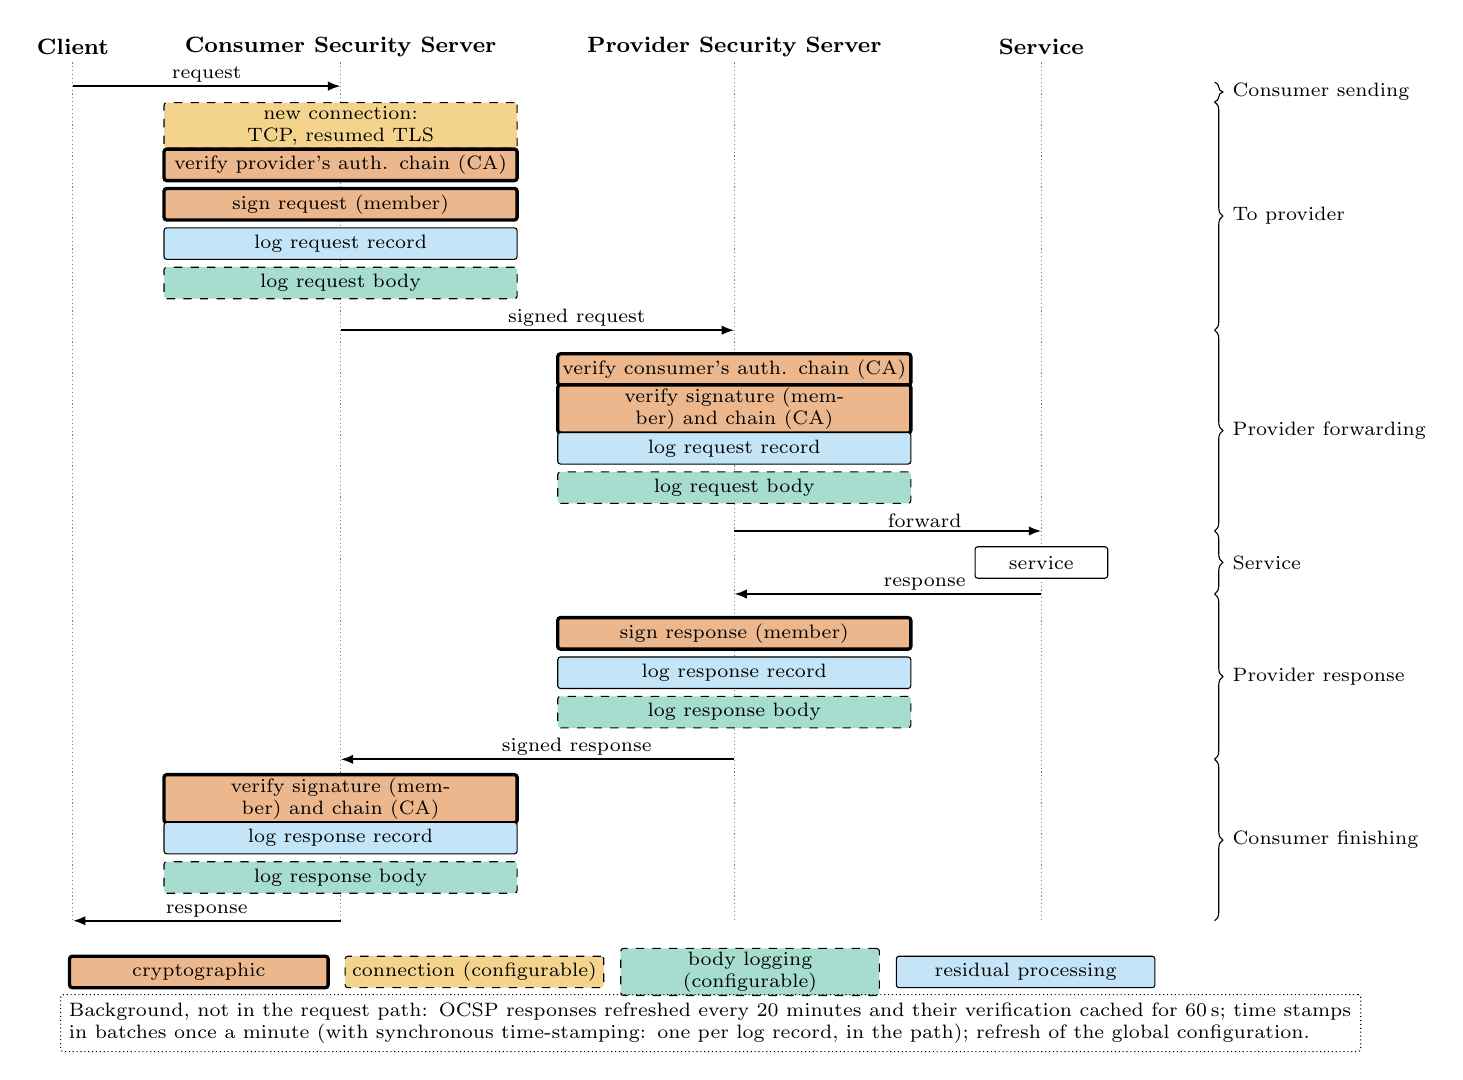
\begin{tikzpicture}[font=\scriptsize, >={Latex[length=1.6mm]},
  box/.style={draw, rounded corners=1pt, minimum height=4mm, text width=4.4cm, align=center,
    inner sep=1.2pt, fill=white},
  crypto/.style={box, very thick, fill=okVermillion!45},
  conn/.style={box, dashed, fill=okOrange!45},
  cfg/.style={box, dashed, fill=okGreen!35},
  fix/.style={box, fill=okSky!35},
  msg/.style={->, thick},
  lbl/.style={above, fill=white, inner sep=1pt}]
% lanes
\foreach \x/\n in {0/Client, 3.4/Consumer Security Server, 8.4/Provider Security Server, 12.3/Service} {
  \node[font=\footnotesize\bfseries] at (\x,0.5) {\n};
  \draw[densely dotted, black!50] (\x,0.3) -- (\x,-10.6);
}
% consumer: request
\draw[msg] (0,0) -- node[lbl]{request} (3.4,0);
\node[conn] at (3.4,-0.5) {new connection: TCP, resumed TLS};
\node[crypto] at (3.4,-1.0) {verify provider's auth. chain (CA)};
\node[crypto] at (3.4,-1.5) {sign request (member)};
\node[fix] at (3.4,-2.0) {log request record};
\node[cfg] at (3.4,-2.5) {log request body};
\draw[msg] (3.4,-3.1) -- node[lbl, pos=0.6]{signed request} (8.4,-3.1);
% provider: request
\node[crypto] at (8.4,-3.6) {verify consumer's auth. chain (CA)};
\node[crypto] at (8.4,-4.1) {verify signature (member) and chain (CA)};
\node[fix] at (8.4,-4.6) {log request record};
\node[cfg] at (8.4,-5.1) {log request body};
\draw[msg] (8.4,-5.65) -- node[lbl, pos=0.62]{forward} (12.3,-5.65);
\node[box, text width=1.6cm] at (12.3,-6.05) {service};
\draw[msg] (12.3,-6.45) -- node[lbl, pos=0.38]{response} (8.4,-6.45);
% provider: response
\node[crypto] at (8.4,-6.95) {sign response (member)};
\node[fix] at (8.4,-7.45) {log response record};
\node[cfg] at (8.4,-7.95) {log response body};
\draw[msg] (8.4,-8.55) -- node[lbl, pos=0.4]{signed response} (3.4,-8.55);
% consumer: response
\node[crypto] at (3.4,-9.05) {verify signature (member) and chain (CA)};
\node[fix] at (3.4,-9.55) {log response record};
\node[cfg] at (3.4,-10.05) {log response body};
\draw[msg] (3.4,-10.6) -- node[lbl, pos=0.5]{response} (0,-10.6);
% stages of operational monitoring
\foreach \a/\b/\l in {0.05/-0.2/Consumer sending, -0.2/-3.1/To provider, -3.1/-5.65/Provider forwarding,
  -5.65/-6.45/Service, -6.45/-8.55/Provider response, -8.55/-10.6/Consumer finishing} {
  \draw[decorate, decoration={brace, amplitude=3pt}] (14.5,\a) -- (14.5,\b)
    node[midway, right=3pt, font=\scriptsize] {\l};
}
% legend and background
\node[crypto, text width=3.2cm] at (1.6,-11.25) {cryptographic};
\node[conn, text width=3.2cm] at (5.1,-11.25) {connection (configurable)};
\node[cfg, text width=3.2cm] at (8.6,-11.25) {body logging (configurable)};
\node[fix, text width=3.2cm] at (12.1,-11.25) {residual processing};
\node[draw, densely dotted, rounded corners=1pt, text width=16.3cm, align=left, inner sep=3pt]
  at (8.1,-11.9) {Background, not in the request path: OCSP responses refreshed every 20 minutes and
  their verification cached for 60\,s; time stamps in batches once a minute (with synchronous time-stamping: one per
  log record, in the path); refresh of the global configuration.};
\end{tikzpicture}
\caption{\newtext{One exchange through X-Road~7.8.3 with the default configuration, from the source
code of the Security Server~\cite{xroadsrc}. Red: cryptographic operations; orange and green,
dashed: steps that configuration changes (the connection policy and the logging of message bodies);
blue: \newtext{residual processing}, which also includes parsing, building and forwarding the messages. On a reused connection the first
two steps of the consumer are skipped. Member: an operation with the member's signing key; CA: the
verification of a CA signature in a certificate chain; auth.: authentication certificate. Braces:
the stages into which the operational monitoring of X-Road divides an exchange.}}
\label{fig:path}
\end{figure*}

The split is a documented design decision: caching status responses and deferring time stamps were
introduced to keep a per-message PKI operation from becoming both a single point of failure and a
latency source~\cite{ansper2013}. It carries a security price as well, since a cached, nonce-less
OCSP response leaves a window during which a revoked certificate is still
accepted~\cite{bakhtina2023ares}. The performance side of that trade-off is the subject of this study.

\newtext{The cost of the trust mechanisms is thus the computation, storage and communication that
the mechanisms described above add to every exchange to establish, validate and preserve evidence
of its authenticity and integrity.} \newtext{Not included in the measured cost are the availability of the trusted services, the issuing
and revocation of certificates, the maintenance of the OCSP cache when responses expire, are missing
or the responder is unavailable, the refresh of the global configuration, full TLS handshakes that
exchange certificates, and key management. Certificate status checking is therefore measured in the
steady state, in which the cache holds valid responses.}

\section{Methodology}

\subsection{Testbed}\label{sec:testbed}

The testbed runs X-Road~7.8.3 in containers built from the official X-Road images: one Central Server, a
test CA that also provides the OCSP and time-stamping services, and four Security Servers --- a
management server, one consumer (\emph{ss1}) and two providers (\emph{ss2}, \emph{ss3}). The measured
path is \emph{load generator $\rightarrow$ ss1 $\rightarrow$ ss2 $\rightarrow$ echo service}; the second
provider is used only to check what limits the consumer under load. The echo service answers a REST
request with a body of the requested size, filled with random bytes so that the message log cannot
compress it, and its own processing time is negligible. The load generator is k6\newtext{~\cite{k6}}, sending REST
\texttt{GET} requests in a closed loop with a given number of concurrent clients, so the message size
below is the size of the response body. The time-stamping service of the test CA was replaced by a
multi-threaded implementation, because the original one handles one request at a time\newtext{, while
synchronous time-stamping sends a request for every record of the message log, so under load the
requests would queue at the service rather than measure the policy}.

Every Security Server is limited to 2 CPU cores and 4\,GB of memory and the Central Server to 2\,GB,
in all environments, so that the environments differ in where the containers run rather than in how
much hardware each of them receives. The whole testbed, including member and service registration,
is set up by scripts from a single composition file and can be redeployed from scratch.

\subsection{Environments}\label{sec:env}

\paragraph{Three machines.} Three identical laptops (Intel Core i5-8250U, 4 cores and 8 threads,
16\,GB of memory) connected by a dedicated wired switch. The first runs the Central Server, the test
CA, the management server and the second provider, the second runs the consumer and the load
generator, and the third runs the provider and the echo service. The containers have their own
addresses on the switch network (Docker \texttt{ipvlan}), so the traffic between the Security
Servers is not translated by the host and leaves the machine. Clocks are synchronised with chrony\newtext{~\cite{chrony}} to
within half a millisecond, which matters when timestamps from two machines are compared.
Figure~\ref{fig:testbed} shows the layout.

\begin{figure}[t]
\centering
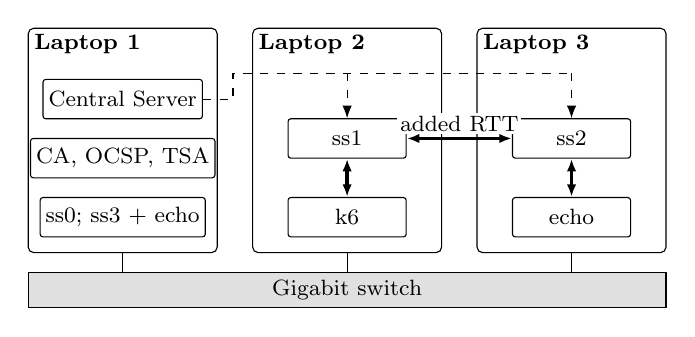
\begin{tikzpicture}[font=\footnotesize, >={Latex[length=1.6mm]},
  c/.style={draw, rounded corners=1pt, minimum height=5mm, align=center, inner sep=2pt, fill=white}]
\foreach \x/\n in {0/1, 2.85/2, 5.7/3} {
  \draw[rounded corners=2pt] (\x,0) rectangle ++(2.4,2.85);
  \node[anchor=north west, inner sep=2pt] at (\x,2.85) {\textbf{Laptop \n}};
  \draw (\x+1.2,0) -- (\x+1.2,-0.25);
}
\draw[fill=black!12] (0,-0.25) rectangle (8.1,-0.7);
\node at (4.05,-0.475) {Gigabit switch};
\node[c, minimum width=2cm] (cs) at (1.2,1.95) {Central Server};
\node[c, minimum width=2cm] (ca) at (1.2,1.2) {CA, OCSP, TSA};
\node[c, minimum width=2cm] at (1.2,0.45) {ss0; ss3 + echo};
\node[c, minimum width=1.5cm] (ss1) at (4.05,1.45) {ss1};
\node[c, minimum width=1.5cm] (k6) at (4.05,0.45) {k6};
\node[c, minimum width=1.5cm] (ss2) at (6.9,1.45) {ss2};
\node[c, minimum width=1.5cm] (echo) at (6.9,0.45) {echo};
\draw[<->, very thick] (k6) -- (ss1);
\draw[<->, very thick] (ss1) -- node[above=1pt, fill=white, inner sep=1pt] {added RTT} (ss2);
\draw[<->, very thick] (ss2) -- (echo);
\draw[dashed] (cs.east) -- (2.6,1.95) -- (2.6,2.28) -- (6.9,2.28);
\draw[dashed, ->] (6.9,2.28) -- (ss2.north);
\draw[dashed, ->] (4.05,2.28) -- (ss1.north);
\end{tikzpicture}
\caption{The testbed on three machines, with the test CA providing OCSP and time-stamping (TSA). Thick line: the measured path. Dashed line: background
traffic to the central services, which is not delayed. All traffic between the Security Servers
passes through the switch.}
\label{fig:testbed}
\end{figure}

\paragraph{One machine.} The same stack on one of these laptops alone. With the same CPU and the
same container limits, the difference to the three-machine environment is the network between the
Security Servers and the sharing of one CPU by all components.

\paragraph{Development laptop.} The same stack on a newer laptop (Intel Core Ultra~7 265U) under
Windows~11, with the containers running in WSL~2. It shows how the absolute numbers depend on the CPU.

\paragraph{Emulated network.} In all of the environments above the Security Servers are at most
one switch apart, with a round-trip time below a millisecond, whereas the Security Servers of two
organisations usually communicate over a longer and less predictable path. From local measurements
alone it is not possible to tell whether the results would hold there. A controlled round-trip time
is therefore added between the consumer and the provider on the three machines with netem, the
network emulator of the Linux kernel~\cite{hemminger2005}, which adds a chosen delay to the packets of
a given flow. This is not a model of a real wide-area deployment, only of the added round-trip time. The same approach is used to study TLS under different network conditions without
Internet-scale infrastructure~\cite{paquin2020}, and the accuracy of the delay netem produces has
been examined in~\cite{nussbaum2009,jurgelionis2011}.

On all machines the CPU runs in its performance power mode, which is checked before every grid and
recorded with it, since the power mode affects the latency.

\subsection{Isolating the cost of a mechanism}\label{sec:iso}

The trust mechanisms of RQ1 cannot all be switched off one at a time, so each of them is observed
in the way that changes as little else as possible (Table~\ref{tab:mech}). \newtext{The architectural
decisions of RQ1 are configuration parameters of X-Road, so their cost is measured by changing them
while the algorithms stay the same.}

\begin{table}[t]
\centering\small
\caption{How the cost of each trust mechanism is observed.}
\label{tab:mech}
\begin{tabular}{@{}p{0.40\columnwidth}p{0.54\columnwidth}@{}}
\toprule
Mechanism & Observed through \\
\midrule
The whole X-Road path & \emph{direct} compared with \emph{full} \\
Inter-server connection policy & \emph{reuse} compared with \emph{full} \\
Logging of message bodies & \emph{nobody} compared with \emph{full} \\
Signing and verification & stages of the \newtext{exchange (Figure~\ref{fig:path})} \\
Time-stamping & requests to the time-stamping service; \emph{synctsa} as another policy \\
Certificate status checking & requests to the OCSP responder \\
\bottomrule
\end{tabular}
\end{table}

Where a setting removes or changes a mechanism, a configuration is compared with the default one
(\emph{full}) and differs from it in that setting only:

\begin{itemize}
  \item \textbf{direct} --- plain HTTP from the load generator to the echo service, without X-Road.
  Its difference to \emph{full} is the whole X-Road path, not any single mechanism.
  \item {\sloppy \textbf{reuse} --- connections between the Security Servers are kept open
  (\param{pool-enable-connection-reuse}, \param{server-support-clients-pooled-connections} and
  \param{server-connector-max-idle-time}). By default each message opens a new
  connection~\cite{xroadsyspar}, so the difference is the effect of the connection policy between
  the Security Servers: setting up the TCP connection and the TLS session and starting every
  transfer on a new TCP connection~\cite{naylor2014}. It does not isolate the TLS handshake.\par}
  \item \textbf{nobody} --- message bodies are not written to the message log
  (\param{message-body-logging=false}), so the difference is the cost of logging the body.
  \item \textbf{synctsa} --- every message is time-stamped synchronously
  (\param{timestamp-immediately=true}). This is a different policy rather than the cost of the
  default batched time-stamping, and is reported as such.
\end{itemize}

Signing and verification cannot be switched off, so they are observed only in the stages of the
\newtext{exchange (Figure~\ref{fig:path})} in which they happen, together with the other work done in the same stages, rather than as
a difference between configurations.

The two background mechanisms cannot be moved into the request path without changing what is
measured. Postponing time stamps by a long interval would violate a documented constraint between the
time-stamping interval and the OCSP freshness~\cite{xroadsyspar}. Making the OCSP freshness shorter
than the interval at which the signer refreshes its cached responses \newtext{would} make every request fail,
because the Security Server takes certificate status only from that cache and does not query the
responder while it processes a message\newtext{~\cite{xroadsrc}}. For these two mechanisms the cost is therefore observed as the number of requests
sent to the time-stamping service and to the OCSP responder during each run and while its messages
are being time-stamped.

\subsection{What is measured}\label{sec:measured}

For each request the load generator records the latency and whether a correct response of the
expected size arrived. For each run the bytes exchanged between consumer and provider,
counted by \texttt{iptables} inside the network namespace of the consumer on the X-Road port, the
growth of the message log, and the number of OCSP and time-stamping requests from the CA log are
recorded.

X-Road also records four timestamps per request on each Security Server in its operational
monitoring database: when the request arrived, when it was forwarded, when the response arrived and
when it was returned. Joining the records of the consumer and the provider by the request identifier
splits the latency into six consecutive stages \newtext{(Figure~\ref{fig:path})}: the consumer before sending, the way to the provider
(the
stage in which signing and logging on the consumer and setting up the connection take place), the
provider before forwarding (the stage in which verification and
logging take place), the echo service, the provider returning the response,
and the consumer finishing it. The stages add up to the time between the request arriving at the
consumer and the response leaving it, which excludes the short way between the load generator and
the consumer. The breakdown is descriptive:
these are timestamps of the measured system itself with a resolution of 1\,ms, and the share of
requests whose records could be matched on both servers is reported with it. Stages measured within
one host are more reliable than the two stages that span hosts, where the residual clock offset enters
the result.

\subsection{Procedure}\label{sec:proc}

Two message sizes are used with one client. Post-quantum signatures and certificates would add a few
kilobytes to every message~\cite{snetkov2023}, which matters most for small messages, so a 10\,KB
response represents a small message; a 1\,MB response represents a large one, whose body the message log stores in full
by default~\cite{xroadsyspar}. One client with no other load gives the baseline latency without
queueing, and the load is then increased until one of the components runs out of
resources~\cite{taklai2020}: the number of clients grows beyond the two CPU cores available to each
Security Server, to 4, 16 and 32, so as to reach the throughput ceiling of the Security Servers; this
range covers the 10 to 30 concurrent clients used in~\cite{taklai2020}. The main grid therefore crosses the five configurations with 10\,KB and 1\,MB
responses at one client and 10\,KB at 4, 16 and 32 clients, plus the two-provider case at 4, 16 and 32 clients.

The Security Server runs on the Java virtual machine, whose first requests after a start are slower
until the code is compiled, so only the steady state is measured~\cite{georges2007}. After every
configuration change the proxy of the Security Servers is restarted and warmed up by a discarded run at four
clients, followed by warm-up requests before every measured run. The amount of warm-up is set from a
pilot run as the point after which the median latency over consecutive windows of requests stops
decreasing. Each run measures 1000 requests, as in~\cite{bakhtina2026ijis}, and 200 at 1\,MB, where
every message adds about a megabyte to the message log of each Security Server.

Following~\cite{georges2007}, every point is measured in several independent runs rather than once.
A grid repeats every point five times; within each repetition plain HTTP runs first, then the
configurations in random order, each with its points in random order, and a control run with the default
configuration at the start of each repetition and at the end shows the drift of the testbed during
the grid. Several grids are run and combined. During the measurements the machines run nothing else. Before the message log is cleaned, the
runner waits until every logged message has its time stamp, so that deferred work is not lost
between runs.

Results are reported as the median over repetitions of each run's median, with the interquartile
range between repetitions and the number of successful requests.

\subsection{Added round-trip time between the Security Servers}\label{sec:delay}

A controlled round-trip time is added between the consumer and the provider with
netem~\cite{hemminger2005}, as done for TLS benchmarking in~\cite{paquin2020}. Half of the
round-trip time is added on each side, in the network namespaces of the two Security Servers and only
for packets to the other server, so that all traffic between them is delayed, including the OCSP
exchange between Security Servers, while the client, the Central Server and the CA stay on the local
network. The delay is fixed, without jitter, since netem reproduces jitter less
accurately~\cite{jurgelionis2011,nussbaum2009}. The results are reported as the effect of a
controlled added round-trip time between the Security Servers, not as a measurement of a real
wide-area deployment. A control at zero delay with the same netem rules installed checks that the
rules themselves do not change the result.

The added round-trip time (0, 5, 20 and 50\,ms) is verified on the measured flow itself: from the
second delay grid on, the round-trip time of the consumer's connections to the provider is read from
the kernel during every run, and a calibration with sequential requests reads it for new connections.
Before the first delay grid, traffic captures of sequential requests on the local network show
whether a request opens a new connection, with a full or a resumed TLS handshake, or uses an existing
one, and how many times one side waits for the other. From these exchanges a prediction is made of how
latency should grow with the round-trip time, and it is compared with the measured slope; where they
disagree, captures under delay are used to find the waits the prediction missed. Captures of a 1\,MB
response with and without connection reuse check how the transfer of a large response depends on the
state of the TCP connection. Since the delay is applied to outgoing packets, they wait inside the
sending host, where they may still count against the limits of the sender's TCP stack on queued data
and so influence how its window grows. As a cross-check, the 1\,MB captures and part of the grid are
repeated with the delay applied to incoming packets on the receiving side instead.

The delay grid crosses \emph{full} and \emph{reuse} with 10\,KB and 1\,MB responses at one client
and 0, 5, 20 and 50\,ms, and an extended grid adds 100\,KB responses and 4 and 16 clients at 0, 20
and 50\,ms. The cross-check grid repeats \emph{full} and \emph{reuse} with 10\,KB and 1\,MB
responses at one client and 0 and 50\,ms.

\subsection{\newtext{Post-quantum signatures}}\label{sec:pqmethod}

{\color{blue}X-Road~7.8.3 has no post-quantum signatures~\cite{bakhtina2026pqc,snetkov2023}, so they
cannot be measured on the testbed directly. A new signature scheme changes two things about a
message: how long it takes to sign and verify it, and how many bytes it has. Studies of
post-quantum TLS separate these two effects: the computation sets the time on fast links, while the
size adds round trips once the data no longer fits into the TCP window, which starts small on a new
connection and grows with every round trip~\cite{paquin2020,sikeridis2020}. The estimate for X-Road
follows the same separation and assumes that the two parts add up. Signing and verification take
time on the CPU of the Security Servers but do not add round trips, because the signatures travel
inside the messages rather than in exchanges of their own (Section~\ref{sec:bg}); the size, in turn,
changes how many round trips the transfer of a message takes on a new connection, which X-Road opens
for every message by default. The computation is therefore measured with a benchmark of the
signature schemes on the Java version and with the cryptographic library that X-Road uses, and the
round trips are derived from the size of the messages and the TCP flights captured in the delay
grids (Section~\ref{sec:delay}). The round-trip part is checked on the testbed with messages padded
to the same size; the assumption that the two parts add up is not checked. \newtext{In other words,
the per-message cost of X-Road is split into terms, and only the terms that depend on the signature
scheme are replaced: the time of signing and verification by the benchmark times of the new scheme,
and the size of the signature parts by their size with the new scheme, whose effect on the round
trips is then measured on X-Road with messages of that size. All other terms, such as logging, the
TLS channel and forwarding, keep the values measured with RSA.} \newtext{Figure~\ref{fig:pqmodel}
shows the two parts of the estimate and its check.}

\begin{figure*}[!tb]
\centering
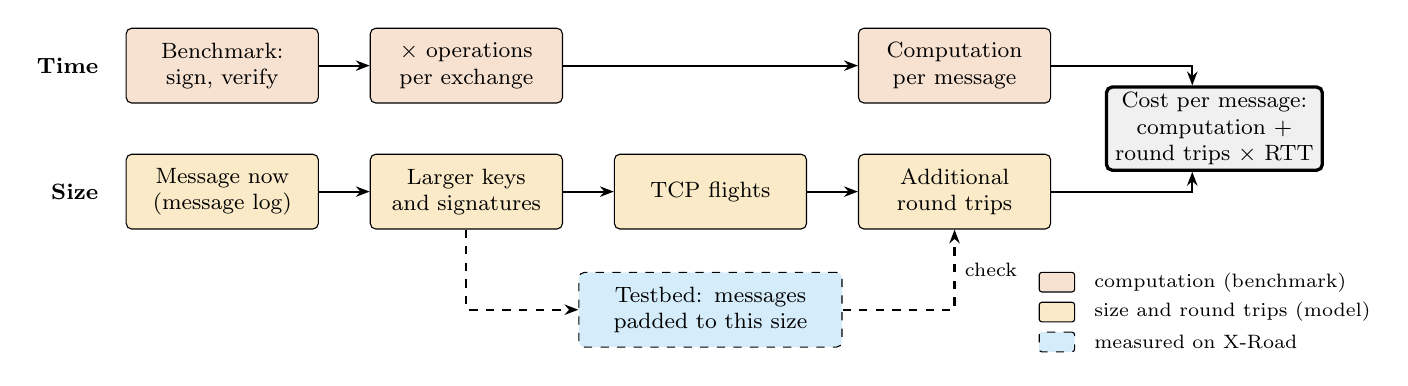
\begin{tikzpicture}[font=\footnotesize,
  box/.style={draw, rounded corners=2pt, align=center, text width=2.3cm, minimum height=0.95cm, inner sep=2pt},
  comp/.style={box, fill=okVermillion!18},
  size/.style={box, fill=okOrange!22},
  check/.style={box, fill=okSky!25, dashed, text width=3.2cm},
  res/.style={box, fill=black!6, very thick, text width=2.6cm},
  arr/.style={-{Stealth[length=5pt]}, thick},
  row/.style={font=\footnotesize\bfseries, anchor=east, align=right}]
\node[row] at (-1.45,0) {Time};
\node[row] at (-1.45,-1.6) {Size};
\node[comp] (c1) at (0,0) {Benchmark:\\sign, verify};
\node[comp] (c2) at (3.1,0) {$\times$ operations\\per exchange};
\node[comp] (c3) at (9.3,0) {Computation\\per message};
\node[size] (s1) at (0,-1.6) {Message now\\(message log)};
\node[size] (s2) at (3.1,-1.6) {Larger keys\\and signatures};
\node[size] (s3) at (6.2,-1.6) {TCP flights};
\node[size] (s4) at (9.3,-1.6) {Additional\\round trips};
\node[res] (e) at (12.6,-0.8) {Cost per message:\\computation $+$\\round trips $\times$ RTT};
\node[check] (k) at (6.2,-3.1) {Testbed: messages\\padded to this size};
\draw[arr] (c1) -- (c2);
\draw[arr] (c2) -- (c3);
\draw[arr] (s1) -- (s2);
\draw[arr] (s2) -- (s3);
\draw[arr] (s3) -- (s4);
\draw[arr] (c3.east) -| ([xshift=-8pt]e.north);
\draw[arr] (s4.east) -| ([xshift=-8pt]e.south);
\draw[arr, dashed] (s2.south) |- (k.west);
\draw[arr, dashed] (k.east) -| node[pos=0.75, right, font=\scriptsize] {check} (s4.south);
\begin{scope}[shift={(10.6,-2.75)}, font=\scriptsize, sw/.style={draw, rounded corners=1pt, minimum width=0.45cm, minimum height=0.25cm, inner sep=0pt}]
\node[sw, fill=okVermillion!18] at (0,0) {}; \node[anchor=west] at (0.35,0) {computation (benchmark)};
\node[sw, fill=okOrange!22] at (0,-0.38) {}; \node[anchor=west] at (0.35,-0.38) {size and round trips (model)};
\node[sw, fill=okSky!25, dashed] at (0,-0.76) {}; \node[anchor=west] at (0.35,-0.76) {measured on X-Road};
\end{scope}
\end{tikzpicture}
\caption{\newtext{How the cost of a post-quantum signature scheme per message is estimated. Time: the signing and verification times
of each scheme from a benchmark outside X-Road, multiplied by the number of these operations in one
exchange. Size: the signature parts of a message with the present
keys, enlarged by the keys and signatures of the new scheme, give the number of TCP flights and so
the round trips added on a new connection. Dashed: the round trips are checked on X-Road with
messages padded to the same size. That the two parts add up is assumed, not checked.}}
\label{fig:pqmodel}
\end{figure*}

\newtext{\paragraph{Scope.} The NIIS report names five areas in which X-Road has to migrate: TLS
between Security Servers and their clients, TLS between two Security Servers, the signing of
messages, the signatures of the global configuration and the signing of time stamps~\cite{bakhtina2026pqc}.
The estimate covers only the signing of messages, including the signatures of the CA and the OCSP
responder that every message carries\newtext{, with one level of CA. The TLS channel between the
Security Servers is left out: X-Road~7.8.3 uses TLS~1.2 only~\cite{xroadsrc}, and the default
configuration resumes its sessions without sending certificates (Figure~\ref{fig:path}). TLS to the
clients is not part of the exchange between Security Servers, and the global configuration and the
time stamps are signed outside the request path (Section~\ref{sec:bg})}.}

\paragraph{Schemes and scenarios.} The schemes are those named in the sources on X-Road and on
post-quantum TLS~\cite{bakhtina2026pqc,snetkov2023,paquin2020,sikeridis2020}: ML-DSA at its three
security levels~\cite{fips204}; Falcon-512 and Falcon-1024, which NIST is standardising as FN-DSA; the
composite signatures that combine ML-DSA with RSA or ECDSA~\cite{rfc10073}, the transition the NIIS
report recommends~\cite{bakhtina2026pqc}; SLH-DSA~\cite{fips205}; and\newtext{, for comparison, ECDSA, which is not
post-quantum but is the only alternative to RSA that X-Road already offers for signing keys (since
version~7.6)~\cite{xroadsyspar}}. The present configuration, RSA-2048 member keys under an
RSA-4096 CA, is the baseline. The parts of a message that depend on the signature scheme fall into
two groups (Section~\ref{sec:bg}): those set by the key of the member, the signature value and the
public key in its certificate, and those set by the keys of the infrastructure, the signature of
the CA on the member's certificate, the signature of the OCSP response, and the key and the CA
signature in the certificate of the OCSP responder. The members and the infrastructure can migrate
separately, so the scenarios differ in which of the two groups uses the new scheme:
\begin{itemize}
  \item \emph{A}: only the member keys change, the CA and the OCSP responder keep RSA-4096;
  \item \emph{B}: the members, the CA and the OCSP responder all use the new scheme;
  \item \emph{C}: the members use ML-DSA, the CA and the OCSP responder use SLH-DSA;
  \item \emph{D}: only the CA and the OCSP responder change, the members keep RSA-2048.
\end{itemize}
SLH-DSA is considered only for the infrastructure (C and D). Its signatures take 7.9 to 30\,KB at the
levels considered~\cite{fips205} and would be carried twice in every exchange, and its signing is
slow: for post-quantum XML signatures it was more than a hundred times slower than that of the other
schemes~\cite{mueller2024}, and with SLH-DSA in the server certificate the TLS handshake became
orders of magnitude slower~\cite{delgado2026}. The CA and the OCSP responder sign rarely and outside
the request path (Section~\ref{sec:bg}), so there only the verification of their signatures is paid
per message.

\paragraph{Computation.} \newtext{Since the schemes are not available in X-Road, their signing and
verification are benchmarked outside it, but in the setting the Security Server would run them in:
with BouncyCastle~1.84\newtext{~\cite{bouncycastle}} on Java~21, the library and Java version of X-Road~7.8.3, which was also used for post-quantum XML signatures~\cite{mueller2024} and was faster
than the native implementation of Java~25 in an earlier JMH study~\cite{oleksiichuk2026}.
X-Road does not sign the message itself: the Security Server builds the
\texttt{SignedInfo} element of an XML signature, which refers to the message only by its digest (in a
batch, by the result of a hash chain), hashes this element and passes the digest to the signer\newtext{~\cite{xroadsrc}}. The signed data is therefore small and does not grow with the
message, while hashing the message itself is the same for every scheme; the benchmark signs a fixed
input of 1\,KB, the order of size of \texttt{SignedInfo}. Since the Java virtual machine compiles code while it runs, a signature
measured right after start is slower than in the steady state of a running Security
Server~\cite{georges2007}, so the benchmark uses JMH\newtext{~\cite{jmh}}, which repeats the operation after a warm-up in
several fresh virtual machines: 5 of them with 10 one-second iterations after 5 warm-up iterations,
and for SLH-DSA-128s and 256s, whose signing is slow~\cite{mueller2024}, 3 with 10 five-second
iterations. \newtext{The benchmark runs on the development laptop (Section~\ref{sec:env}); every
scheme is compared with RSA-2048 on the same CPU, so the comparison depends less on the machine than
the absolute times do. The times of RSA-2048 also give the cost of signing and verification in
X-Road on their own, which the breakdown cannot separate from the other work in its stages
(Section~\ref{sec:iso}).} With one client the operations of an exchange run one after another in the request path, and
the message waits for each of them: the consumer signs the request and, on a new connection,
validates the chain of the provider; the provider verifies the signature of the request and the
chains of the signing and the authentication certificate before forwarding it, and signs the
response; the consumer verifies the response before returning it (Section~\ref{sec:bg}). Their times
therefore add up, and the cost of an exchange is modelled as the sum of the benchmark times over
these operations: two signatures and two verifications with the member key, and four verifications
of a CA signature with \emph{full} and three with \emph{reuse}; the verification of the OCSP response
is cached and not counted. The sum is also the CPU time that the signatures of an exchange take.
Under load the Security Server signs several waiting messages with one signature over a hash
chain~\cite{xroadarcss}, so the cost of signing per message falls; the estimate is made for one
client.} \newtext{Because the signer receives only a digest, while ML-DSA and SLH-DSA in their pure
form sign the data itself, X-Road would need their pre-hash variants, HashML-DSA and
HashSLH-DSA~\cite{fips204,fips205} and the pre-hash composites, or a change of this interface. The
pure and the pre-hash variants of ML-DSA, SLH-DSA-128f and three composites are therefore also
benchmarked side by side in one run with the same settings, to see whether the choice of the
variant changes the time; a pre-hash composite receives the digest of the input, as the signer of
X-Road does.}

\paragraph{Round trips.} The additional round trips are estimated in three steps:
\begin{enumerate}
  \item the size of the signature parts of a request and a response with the present keys
  (Section~\ref{sec:bg}) is measured in the message log of the testbed: the XML signature with the
  signature value, the signing certificate and the OCSP response inside, and the OCSP response for the
  authentication certificate that the request carries;
  \item their size with a new scheme is computed from it: a new scheme enlarges the signature value,
  the member key and the CA signature in the certificate, and the OCSP signature, the responder key and
  the CA signature on the responder certificate, all base64-encoded in the XML, each by the difference
  between the encoded sizes of the new scheme and of RSA;
  \item the number of TCP flights that the larger messages need on a new connection is counted with a
  model whose flight sizes, how many segments the first flight of the request and of the response
  carries and how the following flights grow, are read from the captures of the delay grids
  (Section~\ref{sec:delay}) \newtext{and, where the check below disagrees with the model, from
  captures of the padded messages}.
\end{enumerate}
The model is checked on the testbed by padding the request body and the response to the sizes it
predicts\newtext{. Post-quantum signatures enlarge both the request and the response, since both
carry a signature with the signing certificate and the OCSP response (Section~\ref{sec:bg}). The
\texttt{GET} requests of the other measurements cannot carry this growth: content in a \texttt{GET}
request has no defined meaning in HTTP and a client should not send it~\cite[Sec.~9.3.1]{rfc9110}.
For this check the load generator therefore sends \texttt{POST} requests whose body has the size of
the growth of the request, and the echo service, which returns a body of the requested size
(Section~\ref{sec:testbed}), answers with a response of the predicted size}, with an added
round-trip time of 0 and 50\,ms and, for the largest sizes, 0 and 20\,ms,
with three repetitions per point and 150 requests per run, and with traffic captures where the model
and the testbed disagree. \newtext{Since flight sizes read from a few captures can be off by a segment,
which matters only for a message close to the boundary of a flight, a further grid places points
whose request or response lies within about two segments of a boundary of the model, among them
points of scenario~D, at 0 and 50\,ms.} The delay is added between the two Security Servers in the same way as on
the three machines (Section~\ref{sec:delay}), and the baseline exchange is measured in the same grid,
so that its slope can be compared with that of the three machines. \newtext{The additional round
trips of a point are its median latency at the added round-trip time minus that of the baseline of
the same grid, divided by the round-trip time, so that a shift of the whole machine between grids
cancels. The check runs on the development laptop as well: a round trip counted in this way is set
by TCP rather than by the speed of the CPU.}\par}

\section{Results}

\subsection{Stability of the testbed}

\newtext{In the pilot run the latency did not settle within the first thousand requests after a
restart of the Security Servers, the first run after a restart remained slower even after 4000
requests, and repeated runs at the same point differed by up to 20\,\%; this set the warm-up and the
number of repetitions (Section~\ref{sec:proc}). In the energy-saving power mode of the laptops, in
which an almost idle CPU does not raise its frequency for short bursts of work, the control run took
79.7 instead of 28.7\,ms; all results below were obtained in the performance mode, and the earlier
runs in the energy-saving mode are not used.}

With five repetitions per grid, the main grid was repeated 30 times on three machines (six grids), 15
times on one machine (three grids) and 20 times on the development laptop (four grids). The control run (\emph{full}, 10\,KB response, one
client) had a median of 28.7\,ms over 36 runs on three machines (27.5 to 37.2\,ms, one outlier),
30.4\,ms over 18 runs on one machine (28.9 to 31.2\,ms) and 26.7\,ms over 24 runs on the development
laptop (24.3 to 27.9\,ms). Every request succeeded except in \emph{reuse} under load, where single
requests failed with HTTP~500 in some runs: 7 of 90\,000 requests at 4 to 32 clients on three
machines, 3 of 45\,000 on one machine and 2 of 60\,000 on the development laptop. The failures are
consistent with a pooled connection that was already closed by the other side.

\subsection{\newtext{Division of the path with one client (RQ1)}}\label{sec:rq1}

Table~\ref{tab:onecl} shows the latency with one client. The difference between \emph{direct} and
\emph{full} is the whole X-Road path: on three machines 27.6\,ms for a 10\,KB response and 64\,ms for
a 1\,MB response. Logging the message body makes no difference beyond the spread at 10\,KB, but at
1\,MB not logging it saves 34.9\,ms, 47\,\% of the latency. Keeping connections open between the
Security Servers saves 2.0\,ms at 10\,KB and 4.3\,ms at 1\,MB. Synchronous time-stamping adds
89--92\,ms. The interquartile range between repetitions is 0.7--4.8\,\% of the median on three machines, up
to 9.4\,\% on the development laptop, and up to 5.1\,\% on one machine except for \emph{synctsa}
(18--31\,\%).

\begin{table}[!htb]
\centering\footnotesize
\setlength{\tabcolsep}{3.5pt}
\caption{Median latency with one client (ms) by response size and environment; differences to
\emph{full} in the same environment; Laptop is the development laptop. Every request succeeded.}
\label{tab:onecl}
\begin{tabular}{@{}lrrrrrr@{}}
\toprule
& \multicolumn{2}{c}{3 machines} & \multicolumn{2}{c}{1 machine} & \multicolumn{2}{c}{Laptop} \\
\cmidrule(lr){2-3}\cmidrule(lr){4-5}\cmidrule(l){6-7}
& 10\,KB & 1\,MB & 10\,KB & 1\,MB & 10\,KB & 1\,MB \\
\midrule
\emph{direct} & 0.7 & 10.0 & 0.1 & 0.7 & 0.1 & 0.7 \\
\emph{full} & 28.3 & 74.0 & 29.8 & 74.7 & 24.8 & 49.7 \\
\emph{nobody} $-$ \emph{full} & $-0.9$ & $-34.9$ & $-0.3$ & $-32.0$ & $-0.9$ & $-17.0$ \\
\emph{reuse} $-$ \emph{full} & $-2.0$ & $-4.3$ & $-2.0$ & $-4.3$ & $-1.6$ & $-2.9$ \\
\emph{synctsa} $-$ \emph{full} & $+88.9$ & $+91.7$ & $+91.8$ & $+98.1$ & $+62.4$ & $+68.0$ \\
\midrule
repetitions & \multicolumn{2}{c}{30} & \multicolumn{2}{c}{15} & \multicolumn{2}{c}{20} \\
\bottomrule
\end{tabular}
\end{table}

On three machines a 10\,KB exchange carries 14.8\,KB from consumer to provider and 25.7\,KB back;
with \emph{reuse} 11.5 and 22.8\,KB, so the connection policy costs 3.3 and 2.9\,KB per message in the
two directions. The message log of the consumer grows by 33.7\,KB per exchange with bodies and
19.3\,KB without them, and at 1\,MB by 1.42\,MB and 19.5\,KB.

The two background mechanisms did not appear in the request path. The median number of requests to
the OCSP responder per run was zero; in about 5\,\% of the runs (35 of 741 on three machines) a
background refresh of 2 to 8 requests fell into the run. A configuration with an OCSP freshness
shorter than the refresh of the cached responses made every request fail, as described in
Section~\ref{sec:iso}; this was observed in an early run on the development laptop, but it does not depend on
the power mode. Batched time-stamping sent a median of zero requests to the time-stamping service
during a run (at most two) and about two per run, of about 1200 messages, while the runner waited for
the time stamps; \emph{synctsa} sent 4802 per run, four for each exchange, one for
every record written to the message log.

Table~\ref{tab:stages} shows the per-stage breakdown on three machines. All requests of these runs
were matched between consumer and provider. The stage before the consumer sends the request takes
0.1--0.2\,ms, so the consumer records the request as forwarded when it starts sending, and signing and
logging of the request fall into the stage on the way to the provider. The configurations change the
stages in which their mechanism works: at 10\,KB \emph{reuse} changes only the way to the provider ($-2.4$\,ms);
not logging a 1\,MB body shortens the provider's response by 16.9\,ms and the consumer's finishing
stage by 17.0\,ms, that is, logging the body costs about 17\,ms on each side; and synchronous
time-stamping adds 20--25\,ms to each of the four stages in which a record is logged. The two stages
that span machines include the residual clock offset of below half a millisecond.

\begin{table*}[!b]
\centering\small
\caption{Per-stage breakdown from operational monitoring on three machines, one client (mean of
each run, median over the 15 repetitions of the second series of grids, for which the records of both
servers were kept; ms; resolution 1\,ms). Each column is a median of its own, so the columns
do not add up exactly to the total. ``To provider'' and ``Consumer
finishing'' span two machines.}
\label{tab:stages}
\begin{tabular}{@{}lrrrrrrr@{}}
\toprule
& Consumer & To & Provider & Service & Provider & Consumer & Total \\
& sending & provider & forwarding & & response & finishing & \\
\midrule
\emph{full}, 10\,KB & 0.1 & 10.7 & 4.2 & 0.2 & 6.9 & 7.1 & 29.4 \\
\quad \emph{nobody} $-$ \emph{full} & 0.1 & 0.3 & 0.0 & 0.0 & $-0.8$ & $-0.7$ & $-1.2$ \\
\quad \emph{reuse} $-$ \emph{full} & 0.0 & $-2.4$ & 0.2 & 0.0 & 0.0 & 0.2 & $-2.1$ \\
\quad \emph{synctsa} $-$ \emph{full} & 0.1 & 24.3 & 20.6 & 0.2 & 19.8 & 25.1 & 90.5 \\
\midrule
\emph{full}, 1\,MB & 0.2 & 12.4 & 5.4 & 0.3 & 33.0 & 24.5 & 76.5 \\
\quad \emph{nobody} $-$ \emph{full} & $-0.1$ & $-1.4$ & $-1.2$ & $-0.1$ & $-16.9$ & $-17.0$ & $-37.3$ \\
\quad \emph{reuse} $-$ \emph{full} & 0.0 & $-3.0$ & 0.0 & $-0.1$ & $-1.1$ & 0.0 & $-3.4$ \\
\quad \emph{synctsa} $-$ \emph{full} & 0.1 & 24.5 & 20.9 & 0.2 & 21.8 & 25.0 & 94.5 \\
\bottomrule
\end{tabular}
\end{table*}

{\color{blue}\newtext{Figure~\ref{fig:division}} puts these results together as a division of the X-Road path. The costs that
follow from architectural decisions and can be changed by configuration are small for a 10\,KB
response, 8--11\,\% of the path, and 41--61\,\% of it for a 1\,MB response, mostly because of logging
the body. What remains of the path after them is 22--27\,ms at 10\,KB and grows by 0.1--10.3\,ms
at 1\,MB, while logging the body grows to 17--35\,ms. This remainder contains signing and
verification on both Security Servers, but also logging the message records without bodies
(19.3\,KB per exchange on the consumer), building and parsing the messages and forwarding them, and
these cannot be separated by configuration. The stages that contain signing or verification take
4.2--10.7\,ms each at 10\,KB, which bounds the cryptographic operations from above but does not
measure them alone; their cost alone is measured outside X-Road for RQ3
(Section~\ref{sec:rq3}). The choice between batched and synchronous time-stamping is the largest
architectural decision on the local network: the synchronous policy would add 62--98\,ms, at 10\,KB
\newtext{2.5 to 3.2} times the whole path of the default configuration.\par}

\begin{figure}[!htb]
\centering
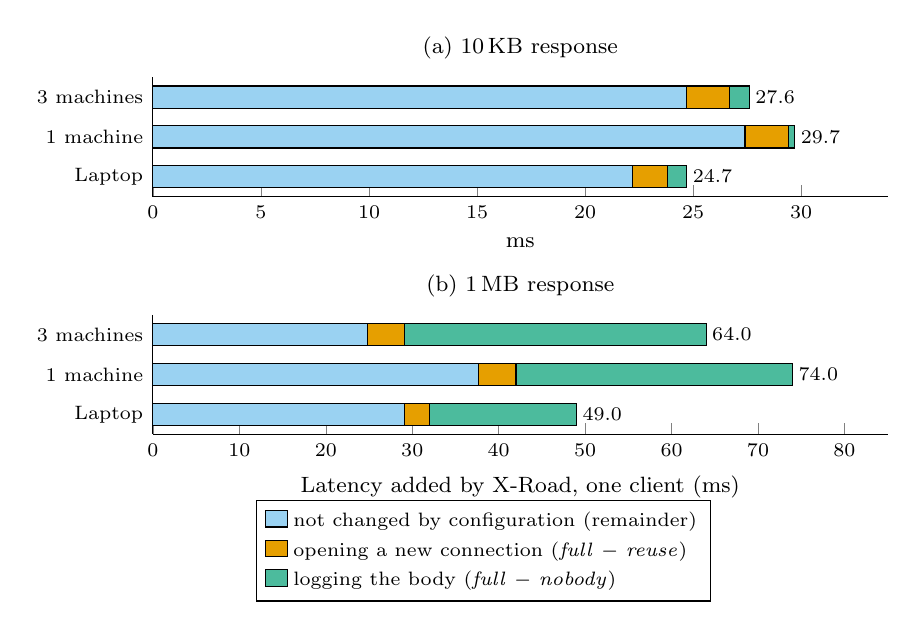
\begin{tikzpicture}
\pgfplotsset{divbar/.style={xbar stacked, width=0.9\columnwidth, height=3.1cm, bar width=8pt,
  xmin=0, clip=false, y dir=reverse, ytick=data, symbolic y coords={T,O,L},
  yticklabels={3 machines, 1 machine, Laptop}, enlarge y limits=0.25,
  axis y line*=left, axis x line*=bottom,
  tick label style={font=\scriptsize}, label style={font=\footnotesize},
  title style={font=\footnotesize, yshift=-3pt}}}
\begin{axis}[divbar, name=small, xmax=34, title={(a) 10\,KB response}, xlabel={ms}]
\addplot[fill=okSky!60, draw=black] coordinates {(24.7,T) (27.4,O) (22.2,L)};
\addplot[fill=okOrange, draw=black] coordinates {(2.0,T) (2.0,O) (1.6,L)};
\addplot[fill=okGreen!70, draw=black] coordinates {(0.9,T) (0.3,O) (0.9,L)};
\node[right, font=\scriptsize, inner sep=2pt] at (axis cs:27.6,T) {27.6};
\node[right, font=\scriptsize, inner sep=2pt] at (axis cs:29.7,O) {29.7};
\node[right, font=\scriptsize, inner sep=2pt] at (axis cs:24.7,L) {24.7};
\end{axis}
\begin{axis}[divbar, at={(small.south west)}, anchor=north west, yshift=-1.5cm, xmax=85,
  title={(b) 1\,MB response}, xlabel={Latency added by X-Road, one client (ms)},
  legend style={font=\scriptsize, at={(0.45,-0.55)}, anchor=north, legend columns=1},
  legend cell align=left]
\addplot[fill=okSky!60, draw=black] coordinates {(24.8,T) (37.7,O) (29.1,L)};
\addlegendentry{not changed by configuration (remainder)}
\addplot[fill=okOrange, draw=black] coordinates {(4.3,T) (4.3,O) (2.9,L)};
\addlegendentry{opening a new connection (\emph{full} $-$ \emph{reuse})}
\addplot[fill=okGreen!70, draw=black] coordinates {(34.9,T) (32.0,O) (17.0,L)};
\addlegendentry{logging the body (\emph{full} $-$ \emph{nobody})}
\node[right, font=\scriptsize, inner sep=2pt] at (axis cs:64.0,T) {64.0};
\node[right, font=\scriptsize, inner sep=2pt] at (axis cs:74.0,O) {74.0};
\node[right, font=\scriptsize, inner sep=2pt] at (axis cs:49.0,L) {49.0};
\end{axis}
\end{tikzpicture}
\caption{\newtext{Division of the X-Road path with one client, from Table~\ref{tab:onecl}. A bar is
the whole path, \emph{full} $-$ \emph{direct}, with its length in ms; the remainder contains signing,
verification and the other processing of the Security Servers. The scales of (a) and (b) differ.
Synchronous time-stamping, not in the default, would add another 62--98\,ms
(\emph{synctsa} $-$ \emph{full}).}}
\label{fig:division}
\end{figure}


\subsection{Response size and load (RQ2)}

From a 10\,KB to a 1\,MB response, the latency of \emph{full} on three machines grows from 28.3 to
74.0\,ms, while \emph{direct} grows from 0.7 to 10.0\,ms. Without body logging the growth is from 27.4
to 39.1\,ms, so most of the additional time at 1\,MB is writing the body to the message log. The
effect of the connection policy grows from 2.0 to 4.3\,ms, and the cost of synchronous time-stamping
stays at about 90\,ms. \newtext{With size the division therefore shifts towards the architecture: the
remainder of the path grows by at most 10\,ms, while logging the body grows to 17--35\,ms
(\newtext{Figure~\ref{fig:division}}).}

Under load the spread between repetitions grows to 9--41\,\% of the throughput for \emph{full},
\emph{nobody}, \emph{reuse} and the two-provider case across the environments (15--41\,\% on three
machines), while for \emph{synctsa} it stays at 4--10\,\% except at four clients on one machine
(20\,\%).
Table~\ref{tab:load} therefore lists the highest throughput each configuration reached. The
differences between \emph{full}, \emph{nobody}, \emph{reuse} and two providers are within the spread
and are not assigned to individual mechanisms. Synchronous time-stamping halves the ceiling on three
machines (50 against 106 requests per second)\newtext{, and lowers it to 37\,\% on one machine (28 against 75) and on the development laptop (41 against 112)}. A second provider does not raise the ceiling either:
with two providers the stages of each provider become shorter, but the consumer's finishing stage
becomes longer, so \newtext{in this two-provider configuration} the consumer is the limit.

\begin{table}[!htb]
\centering\footnotesize
\setlength{\tabcolsep}{4pt}
\caption{Highest median throughput reached at 4, 16 or 32 clients, 10\,KB response (requests per
second); in brackets the number of clients at which it was reached and the interquartile range of
the throughput between repetitions (\%).}
\label{tab:load}
\begin{tabular}{@{}lccc@{}}
\toprule
& 3 machines & 1 machine & Laptop \\
\midrule
\emph{full} & 106 (16; 32) & 75 (32; 29) & 112 (32; 9) \\
\emph{nobody} & 106 (32; 19) & 76 (16; 17) & 107 (32; 15) \\
\emph{reuse} & 108 (16; 21) & 79 (16; 20) & 118 (32; 15) \\
two providers & 111 (32; 24) & 82 (16; 36) & 109 (32; 24) \\
\emph{synctsa} & 50 (16; 10) & 28 (32; 5) & 41 (32; 5) \\
\bottomrule
\end{tabular}
\end{table}

\subsection{Environment and added round-trip time \newtext{(RQ2)}}\label{sec:rtt}

With one client, three machines and one machine give the same picture (Table~\ref{tab:onecl}): the
latency of \emph{full} differs by 0.7--1.5\,ms and the differences between configurations by at most
6.4\,ms.
\emph{direct} shows that the switch adds 0.6\,ms at 10\,KB and 9.3\,ms at 1\,MB, but through X-Road
this is offset by the provider having a CPU of its own: on three machines the provider's stages are
shorter (4.2 against 5.7\,ms and 6.9 against 9.0\,ms), while the way to the provider is 0.6\,ms longer.
Under load three machines reach 1.4 to 1.8 times higher throughput (Table~\ref{tab:load}), because the
work is spread over three CPUs. With one client, all absolute values on the development laptop are lower and the
CPU-bound costs smaller (logging a 1\,MB body 17 instead of 35\,ms, synchronous time-stamping 62
instead of 89\,ms), while the differences keep their sign and order.

\paragraph{Added round-trip time.} In the three delay grids in which it was recorded,
the round-trip time of the connections between the Security Servers, as smoothed by the kernel (which
includes delayed acknowledgements), was 0.5, 6.1, 21.4 and 51.5\,ms for \emph{full} and 2.7, 8.1,
23.5 and 54.2\,ms for \emph{reuse} at an added 0, 5, 20 and 50\,ms; in a calibration with sequential
requests the minimum for new connections was 0.53, 5.54, 20.78 and 51.11\,ms. With the netem rules installed and no delay, the latency did not change at
10\,KB (31.0 against 30.6\,ms for \emph{full}, 27.7 against 28.9\,ms for \emph{reuse}); at 1\,MB it
was 3--4\,ms higher (about 5\,\%, with overlapping ranges), one to two orders of magnitude below the
effect of the added round-trip time (47\,ms for \emph{full} at 1\,MB already at 5\,ms).

Before the first grid with added delay, traffic captures on the local network showed that every
message of \emph{full} opens a new TCP connection and resumes the TLS~1.2 session from a session
ticket, without exchanging certificates. Counting the TCP handshake, the TLS handshake and the
request itself, a message of \emph{full} waits for three round trips between the Security Servers
and a message of \emph{reuse} for one. The growth of latency is therefore described by its slope
against the added round-trip time: a slope of 3 means that the latency grows by three times the added
round-trip time, that is, every message waits for three round trips. It is computed from the medians at 0 and
50\,ms. The prediction was a slope of 3
for \emph{full} and 1 for \emph{reuse}. Figure~\ref{fig:rtt} and Table~\ref{tab:rtt} show the measurement: at 10\,KB the
slope is 5.1 for \emph{full} and 2.1 for \emph{reuse}, so the prediction underestimated both.
Captures under delay showed two waits it did not include: the last part of the request (842 bytes
after about 10\,KB) is held until the provider acknowledges the earlier data, which adds one round
trip in both configurations, and on a new connection the response of about 26\,KB does not fit into
the initial TCP window and needs a second flight, which adds one more round trip to \emph{full}\newtext{:
the response starts with small TLS records, the start of the MIME message and the delimiters of
its chunks, sent as one packet each, which use up the initial window, and the body follows only
after an acknowledgement}. With
these, the count is 5 and 2; a calibration with sequential requests on the three machines gave
slopes of 4.7 and 1.9. A short wait inside the TLS handshake, between the message that switches the
consumer to the negotiated keys and its first encrypted message, appeared at 20\,ms and not at
50\,ms and causes a variation of about 0.3--0.4 in the slope. The stage breakdown agrees: the slope of
the way to the provider is 2.6 for \emph{full} and 0.5 for \emph{reuse}, and that of the provider's
forwarding stage is 1 in both.

\begin{figure}[!htb]
\centering
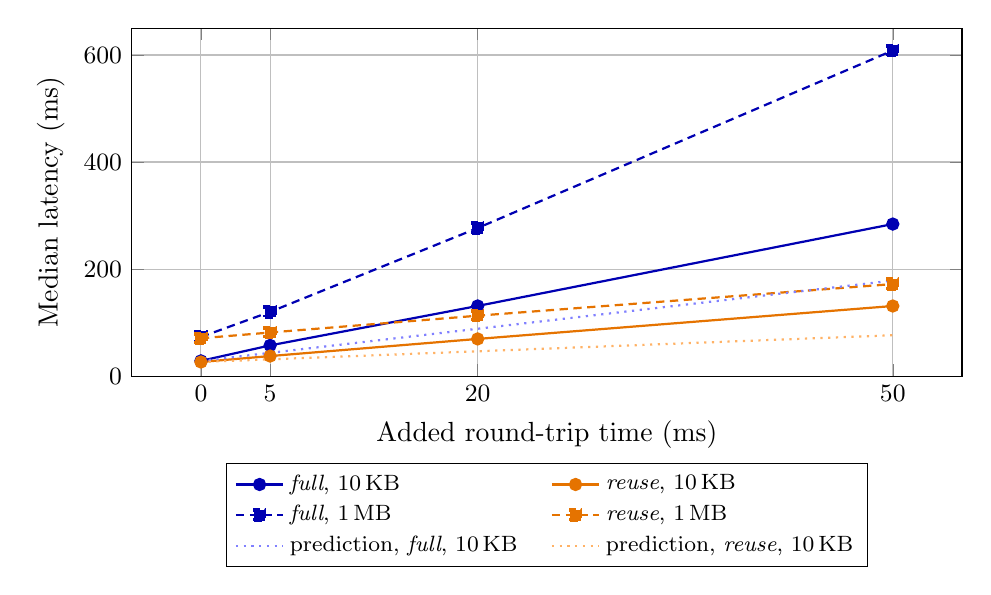
\begin{tikzpicture}
\begin{axis}[width=\columnwidth, height=6cm, xlabel={Added round-trip time (ms)},
  ylabel={Median latency (ms)}, xtick={0,5,20,50}, ymin=0, ymax=650, grid=major,
  legend style={font=\footnotesize, at={(0.5,-0.25)}, anchor=north, legend columns=2,
  /tikz/every even column/.append style={column sep=1em}}, legend cell align=left,
  tick label style={font=\small}]
\addplot[mark=*, thick, blue!70!black] coordinates {(0,28.5) (5,57.4) (20,131.1) (50,284.1)};
\addlegendentry{\emph{full}, 10\,KB}
\addplot[mark=*, thick, orange!90!black] coordinates {(0,26.4) (5,37.5) (20,69.5) (50,131.0)};
\addlegendentry{\emph{reuse}, 10\,KB}
\addplot[mark=square*, thick, densely dashed, blue!70!black] coordinates {(0,73.1) (5,120.0) (20,276.7) (50,608.4)};
\addlegendentry{\emph{full}, 1\,MB}
\addplot[mark=square*, thick, densely dashed, orange!90!black] coordinates {(0,70.7) (5,81.5) (20,112.9) (50,172.0)};
\addlegendentry{\emph{reuse}, 1\,MB}
\addplot[dotted, thick, blue!50, domain=0:50, samples=2] {28.5+3*x};
\addlegendentry{prediction, \emph{full}, 10\,KB}
\addplot[dotted, thick, orange!60, domain=0:50, samples=2] {26.4+1*x};
\addlegendentry{prediction, \emph{reuse}, 10\,KB}
\end{axis}
\end{tikzpicture}
\caption{Latency with one client against the round-trip time added between the Security Servers,
three machines, 20 repetitions; lines without
marks show the prediction made before the measurement.}
\label{fig:rtt}
\end{figure}

\begin{table*}[!tb]
\centering
\caption{The points of Figure~\ref{fig:rtt}: median latency over 20 repetitions (ms), in brackets the
first and third quartiles of the run medians.}
\label{tab:rtt}
\setlength{\tabcolsep}{4pt}
\begin{tabular}{@{}lcccc@{}}
\toprule
& 0\,ms & 5\,ms & 20\,ms & 50\,ms \\
\midrule
\emph{full}, 10\,KB & 28.5 (27.9--28.7) & 57.4 (57.0--57.9) & 131.1 (130.9--131.4) & 284.1 (283.6--284.3) \\
\emph{reuse}, 10\,KB & 26.4 (26.1--26.7) & 37.5 (37.0--37.6) & 69.5 (69.2--69.7) & 131.0 (130.7--131.1) \\
\emph{full}, 1\,MB & 73.1 (71.5--76.1) & 120.0 (118.6--121.8) & 276.7 (275.6--281.1) & 608.4 (607.3--610.4) \\
\emph{reuse}, 1\,MB & 70.7 (68.3--72.9) & 81.5 (80.0--82.8) & 112.9 (110.9--115.0) & 172.0 (170.3--173.7) \\
\bottomrule
\end{tabular}
\end{table*}

At 1\,MB the slope is 10.7 for \emph{full} and 2.0 for \emph{reuse}.
Captures of a 1\,MB response at 50\,ms show the reason: on a new connection the body leaves in about
six flights, one per round trip, each about twice as large as the previous one (28, 57, 113, 226 and
453\,KB), as the TCP window grows from its initial size; with \emph{reuse} the window is kept between
messages and keeps growing, so the response leaves in fewer flights, and from the fifth request on
in one flight. The effect of the
connection policy thus grows from 2\,ms on the local network to 153\,ms (54\,\%) at 10\,KB and
436\,ms (72\,\%) at 1\,MB with an added 50\,ms.

The extended grid confirms the pattern. With a 100\,KB response the slope is 7.0 for \emph{full} and
2.1 for \emph{reuse}, so with a new connection for every message the cost of distance grows with the
size of the response (slopes of 5.0, 7.0 and 9.7 for 10\,KB, 100\,KB and 1\,MB in this grid), while
with reused connections it does not. The slope at 1\,MB is lower here than in the first delay grid
(9.7 against 10.7) because the medians of the two series differ by 8\,ms at 0\,ms and by 45\,ms at
50\,ms; at 10\,KB the two grids agree (5.0 and 5.1). With an added round-trip time the
latency with four clients is the same as with one, and at 50\,ms throughput is limited by the round trips: 14 requests per second for
\emph{full} against 30 for \emph{reuse}. With 16 clients at 0 and 20\,ms the Security Servers are the
limit (103--127 requests per second) and the added round-trip time disappears in the queue (142
against 140\,ms for \emph{full}); at 50\,ms \emph{full} falls to 57 requests per second while
\emph{reuse} keeps 104. Errors again occurred only with \emph{reuse} under load: 17 of 90\,000
requests at 4 and 16 clients.

With the delay applied to incoming instead of outgoing packets the slopes are the same: 5.0 for
\emph{full} and 2.1 for \emph{reuse} at 10\,KB, and 9.6 and 2.0 at 1\,MB (15 repetitions, no
errors). Captures of a 1\,MB response at 50\,ms show the same flights on a new connection (28, 57,
113, 226 and 453\,KB), and with \emph{reuse} the window is again kept between messages. The slope
of \emph{full} at 1\,MB therefore does not depend on where the delay is applied: it agrees with the
extended grid (9.7), while the first delay grids gave 10.7, so between nights it varies by about one
round trip.

{\color{blue}With distance the division shifts further. Signatures travel inside the messages, so signing and
verification add no round trips of their own, and in the stage breakdown most of the round trips fall into the
way to the provider and the provider's forwarding stage, where the connection is set up and the
request is transferred. The round trips are decided by the connection policy and by how TCP transfers
a message on a new connection: at an added 50\,ms the connection policy costs 153\,ms at 10\,KB and
436\,ms at 1\,MB, against a remainder of about 25\,ms on the same three machines without added delay.

\subsection{\newtext{Post-quantum signatures (RQ3)}}\label{sec:rq3}

\newtext{Table~\ref{tab:pq} shows the benchmark and the estimate for each scheme
(Section~\ref{sec:pqmethod}). One signature with SLH-DSA took 32\,ms to 1.1\,s. The verification of
RSA-4096, the key of the test CA, took 85\,$\mu$s. In the message log of the testbed the
\texttt{SignedInfo} element took 813 bytes in a request and 825 bytes in a response, so the input of
the benchmark is close to what X-Road signs. On the development laptop the baseline exchange with a
10\,KB response and \emph{full} had a slope of 5.4 against the added round-trip time, against 5.1 on
the three machines (Table~\ref{tab:rtt}), and the captures on both showed the same sequence of
flights, so the round trips counted on the laptop apply to the three machines as well. The error of the mean (99.9\,\% interval) was at
most 4\,\% except for signing with ML-DSA and its composites with ECDSA (11 to 35\,\%), since signing
with ML-DSA repeats a random number of attempts.}

\newtext{With the present keys the XML signature of a request took 7969 bytes and that of a response
8002 bytes, and the OCSP response for the authentication certificate 2052 bytes. In the captures of
the delay grids a new connection started with a window of 10 segments,
the first flight of the \newtext{baseline} request after the handshake carried \newtext{8} of them, the start of the response
consisted of small TLS records that used up the initial window (Section~\ref{sec:rtt}), and each
further flight doubled; the \newtext{first version of the} model counts flights with these sizes. In the check of the round-trip
model on the testbed one request of about \newtext{60\,600} failed. The largest
request needed one flight more than the first version of the model predicted. A capture \newtext{of
this padded request} showed that
from the fourth flight on the request is limited by the receive window of the provider (about
95\,KB, so 36 and 41 segments instead of 80), not by the congestion window; the model was corrected
accordingly\newtext{. The grid near the flight boundaries showed one more disagreement: a request of
41\,315 bytes on the wire (B, ML-DSA-65 + P-256) needed two flights, not three. \newtext{In the
captures of the padded requests the first flight carried 9 full segments. The baseline request fits
into it, but its last, partial segment left only after an acknowledgement, like the last part of
the request in Section~\ref{sec:rtt}, for a reason the captures do not show; this flight therefore held only 8 full
segments.} The model now counts 9 segments in the
first flight and at least two flights per request}, and \newtext{Figure~\ref{fig:flights}b}
compares the corrected model with the testbed.}

\begin{table*}[!tb]
\centering\footnotesize
\caption{Signature schemes on the development laptop and their estimated cost per message against the
baseline (RSA-2048 members, RSA-4096 CA). Computation: change of the signing and verification time
of one exchange with \emph{full} (baseline 1.7\,ms)\newtext{, rounded to 0.1\,ms; the error of the
mean of signing with ML-DSA and its composites (99.9\,\% interval) amounts to up to $\pm$0.4\,ms per
exchange}. Size: bytes added to the request and the
response. Round trips: additional round trips of one exchange with \emph{full}; with \emph{reuse} none
in any row. For SLH-DSA, scenario C: members ML-DSA-65, CA and OCSP responder SLH-DSA.}
\label{tab:pq}
\color{blue}
\setlength{\tabcolsep}{3.5pt}
\begin{tabular}{@{}lrrrrrrrrrr@{}}
\toprule
& & & & & \multicolumn{3}{c}{A: member keys} & \multicolumn{3}{c}{B, C: members, CA, OCSP} \\
\cmidrule(lr){6-8}\cmidrule(l){9-11}
Scheme & Key (B) & Signature (B) & Sign ($\mu$s) & Verify ($\mu$s) & Comp.\ (ms) & Size (KB) & RTT
& Comp.\ (ms) & Size (KB) & RTT \\
\midrule
RSA-2048 (baseline) & 294 & 256 & 668 & 26 & --- & --- & --- & --- & --- & --- \\
ECDSA P-256 & 91 & 70--72 & 54 & 52 & \newtext{$-1.2$} & $-0.6$ / $-0.6$ & 0 & \newtext{$-1.3$} & $-4.5$ / $-3.1$ & \newtext{0} \\
ML-DSA-44 & 1334 & 2420 & 202 & 61 & \newtext{$-0.9$} & 4.6 / 4.6 & 0 & \newtext{$-1.0$} & 18.6 / 14.0 & 1 \\
ML-DSA-65 & 1974 & 3309 & 314 & 96 & \newtext{$-0.6$} & 6.8 / 6.8 & 0 & \newtext{$-0.5$} & 27.9 / 20.9 & 1 \\
ML-DSA-87 & 2614 & 4627 & 462 & 158 & \newtext{$-0.1$} & 9.6 / 9.6 & 1 & \newtext{$+0.1$} & 40.6 / 30.4 & 2 \\
Falcon-512 & 915 & 650--662 & 259 & 26 & \newtext{$-0.8$} & 1.5 / 1.5 & 0 & \newtext{$-1.1$} & \newtext{3.3 / 2.7} & 0 \\
Falcon-1024 & 1811 & 1261--1277 & 519 & 52 & \newtext{$-0.2$} & 3.7 / 3.7 & 0 & \newtext{$-0.4$} & 11.6 / 8.8 & 1 \\
ML-DSA-44 + RSA-2048 & 1603 & 2676 & 881 & 90 & \newtext{$+0.6$} & 5.4 / 5.4 & 0 & \newtext{$+0.6$} & 21.6 / 16.2 & 1 \\
ML-DSA-44 + P-256 & 1398 & 2489--2492 & 359 & 114 & \newtext{$-0.4$} & 4.8 / 4.8 & 0 & \newtext{$-0.3$} & 19.4 / 14.6 & 1 \\
ML-DSA-65 + RSA-3072 & 2371 & 3693 & 2191 & 147 & \newtext{$+3.3$} & 7.9 / 7.9 & 0 & \newtext{$+3.5$} & 32.5 / 24.3 & 2 \\
ML-DSA-65 + P-256 & 2038 & 3378--3381 & 302 & 150 & \newtext{$-0.5$} & 7.0 / 7.0 & 0 & \newtext{$-0.2$} & 28.8 / 21.5 & \newtext{1} \\
ML-DSA-87 + RSA-4096 & 3139 & 5139 & 4782 & 243 & \newtext{$+8.7$} & 11.1 / 11.1 & 1 & \newtext{$+9.3$} & 46.7 / 34.8 & 2 \\
ML-DSA-87 + P-384 & 2710 & 4729--4731 & 662 & 325 & \newtext{$+0.6$} & 9.9 / 9.9 & 1 & \newtext{$+1.5$} & 41.8 / 31.2 & 2 \\
SLH-DSA-128s & 50 & 7856 & 704\,547 & 619 & --- & --- & --- & \newtext{$+1.6$} & 52.0 / 37.8 & 2 \\
SLH-DSA-128f & 50 & 17\,088 & 31\,957 & 1819 & --- & --- & --- & \newtext{$+6.4$} & 110.3 / 77.6 & 4 \\
SLH-DSA-256s & 82 & 29\,792 & 1\,088\,102 & 1363 & --- & --- & --- & \newtext{$+4.5$} & 190.6 / 132.5 & 5 \\
\bottomrule
\end{tabular}
\end{table*}

\begin{figure*}[!tb]
\centering
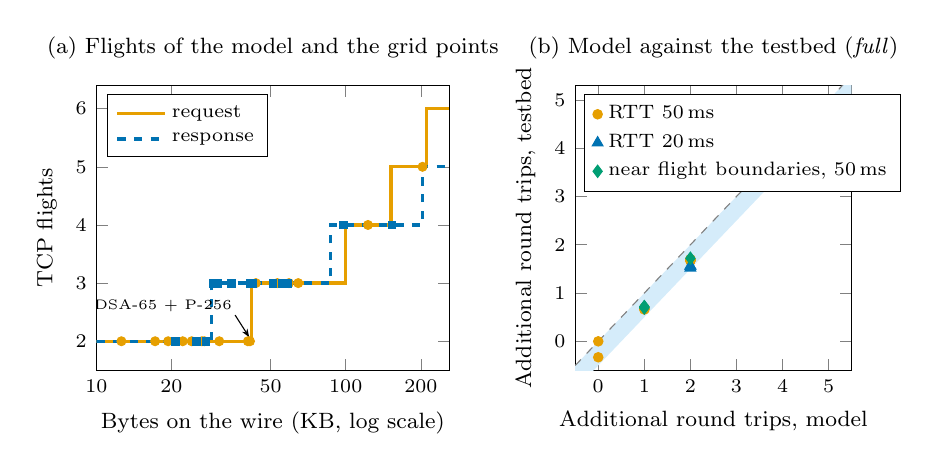
\begin{tikzpicture}
\begin{axis}[name=fa, width=0.5\textwidth, height=5.2cm, xmode=log, log basis x=10,
  xmin=10, xmax=260, ymin=1.5, ymax=6.4, ytick={2,3,4,5,6},
  xtick={10,20,50,100,200}, xticklabels={10,20,50,100,200},
  xlabel={Bytes on the wire (KB, log scale)}, ylabel={TCP flights},
  title={(a) Flights of the model and the grid points}, title style={font=\footnotesize},
  tick label style={font=\scriptsize}, label style={font=\footnotesize},
  legend style={font=\scriptsize, at={(0.03,0.97)}, anchor=north west}, legend cell align=left]
\addplot[const plot, very thick, okOrange] coordinates {(10,2) (41.992,3) (99.912,4) (152.04,5) (211.408,6) (260,6)};
\addlegendentry{request}
\addplot[const plot, very thick, okBlue, dashed] coordinates {(10,2) (28.96,3) (86.88,4) (202.72,5) (260,5)};
\addlegendentry{response}
\addplot[only marks, mark=*, mark size=1.6pt, okOrange, forget plot] coordinates {(12.6,2) (17.2,2) (19.4,2) (22.2,2)
  (31.1,2) (40.5,2) (53.2,3) (59.2,3) (64.5,3) (122.8,4) (203.2,5) (24.1,2) (41.3,2) (26.5,2) (27.1,2) (43.6,3)};
\addplot[only marks, mark=square*, mark size=1.4pt, okBlue, forget plot] coordinates {(20.7,2) (25.3,2) (27.5,2) (30.3,3)
  (34.7,3) (41.6,3) (51.1,3) (55.5,3) (58.5,3) (98.3,4) (153.2,4) (29.5,3) (42.2,3) (30.1,3) (30.5,3) (41.4,3)};
\node[font=\tiny, anchor=south east, inner sep=1pt] (lb) at (axis cs:36,2.45) {B ML-DSA-65 + P-256};
\draw[-{Stealth[length=3pt]}] (lb.south east) -- (axis cs:41.0,2.07);
\end{axis}
\begin{axis}[at={(fa.east)}, anchor=west, xshift=1.6cm, width=0.42\textwidth, height=5.2cm,
  xmin=-0.5, xmax=5.5, ymin=-0.6, ymax=5.3, xtick={0,1,2,3,4,5}, ytick={0,1,2,3,4,5},
  xlabel={Additional round trips, model}, ylabel={Additional round trips, testbed},
  title={(b) Model against the testbed (\emph{full})}, title style={font=\footnotesize},
  tick label style={font=\scriptsize}, label style={font=\footnotesize},
  legend style={font=\scriptsize, at={(0.03,0.97)}, anchor=north west}, legend cell align=left]
\addplot[fill=okSky!25, draw=none, forget plot] coordinates {(-0.5,-1) (5.5,5) (5.5,5.5) (-0.5,-0.5)} -- cycle;
\addplot[black!50, dashed, forget plot] coordinates {(-0.5,-0.5) (5.5,5.5)};
\addplot[only marks, mark=*, mark size=1.7pt, okOrange] coordinates {(0,0.00) (1,0.69) (0,-0.33) (1,0.66) (1,0.67)
  (2,1.70) (2,1.67) (2,1.69) (2,1.68) (4,3.74) (5,4.65) (2,1.68) (2,1.68) (2,1.69) (4,3.70) (5,4.65)};
\addlegendentry{RTT 50\,ms}
\addplot[only marks, mark=triangle*, mark size=2.2pt, okBlue] coordinates {(2,1.52) (2,1.56) (2,1.56) (4,3.85) (5,4.81)};
\addlegendentry{RTT 20\,ms}
\addplot[only marks, mark=diamond*, mark size=2.2pt, okGreen] coordinates {(1,0.71) (1,0.71) (1,0.72) (2,1.72) (1,0.69)};
\addlegendentry{near flight boundaries, 50\,ms}
\end{axis}
\end{tikzpicture}
\caption{\newtext{The model of the TCP flights (Section~\ref{sec:pqmethod}) and its check, new
connection (\emph{full}). (a) Flights that the model counts for a request (TLS bytes after the
handshake) and for a response (bytes after its first flight of small records; that flight is
counted) of a given size; the points are the 16 sizes of the grids, each on its two lines. Point B
ML-DSA-65 + P-256 lies 0.7\,KB below a boundary of the request; the first version of the model,
with a first flight of 8 segments, put it above. (b) Additional round trips counted by the model
against those measured, \newtext{the median latency at the added round-trip time minus that of the
baseline, divided by the round-trip time}\newtext{, one value per grid}; 26 points.
Shaded: up to half a round trip below the model, the part of a round trip that the baseline already
waits (Section~\ref{sec:rtt}).}}
\label{fig:flights}
\end{figure*}

\newtext{The computation changes little (Table~\ref{tab:pq}). Without RSA, the signatures of an
exchange take from 1.3\,ms less than with RSA-2048 to about the same, because signing with RSA is
the most expensive operation of the baseline; only ML-DSA-87 + P-384 adds up to 1.5\,ms. The
composites with RSA keep the cost of their RSA half: about 0.6\,ms more with RSA-2048 and 3.3 to
9.3\,ms with RSA-3072 and RSA-4096. SLH-DSA in the role of the CA adds 1.6 to 6.4\,ms, because its
signature is verified in every message.} The whole signing and verification of the
baseline, 1.7\,ms, is 7\,\% of the 24.7\,ms that the X-Road path takes on the same laptop
(\newtext{Figure~\ref{fig:division}}). \newtext{These times hold for the development laptop. On the three
machines the costs that depend on the CPU were 1.4 to 2.1 times higher (synchronous time-stamping 89
against 62\,ms, logging a 1\,MB body 35 against 17\,ms, Table~\ref{tab:onecl}). Scaled by these
factors, the signatures of the baseline would take 2.4 to 3.5\,ms there, and the composites with
RSA-3072 and RSA-4096 and SLH-DSA in the CA would add up to 13 to 19\,ms instead of up to 9.3\,ms,
comparable with the remainder of the path of 24.7\,ms on the same machines; for ML-DSA and Falcon
the change stays within about 1\,ms.}

\newtext{The pre-hash variants take the same time as the pure ones. In the run that measured both
side by side, verification differed by at most 7\,$\mu$s (0.4\,\% with SLH-DSA-128f, 1 to 5\,\% with
ML-DSA and the composites), signing with ML-DSA and the composites by at most 83\,$\mu$s, within the
error of the mean of this signing, which repeats a random number of attempts, and signing with
SLH-DSA-128f, which only the CA and the OCSP responder do, by 0.9\,\%. For the two
signatures and two verifications with the member key in an exchange this is less than 0.2\,ms, so the
estimates of Table~\ref{tab:pq}, made with the pure variants, hold for the pre-hash variants that the
interface of the signer of X-Road would need.}

The size matters only on a new connection. When only the member keys change (A), the messages grow by
1.5 to 11\,KB and need no additional round trip, except with ML-DSA-87 \newtext{and its two composites}, where the response no longer
fits into its second flight. When the CA and the OCSP responder change as well (B), the certificates
and the OCSP responses in every message grow too, and the messages grow by 3 to 47\,KB: one additional
round trip with ML-DSA-44, ML-DSA-65, Falcon-1024\newtext{,} the composites of ML-DSA-44 \newtext{and
ML-DSA-65 + P-256}, two with ML-DSA-87\newtext{, ML-DSA-65 + RSA-3072} and the composites of
ML-DSA-87\newtext{; with ECDSA, which makes the messages smaller, the number of flights stays the same}. Falcon-512 is the only post-quantum scheme that needs none in \newtext{any} scenario. With SLH-DSA
for the CA the messages grow by 52 to 191\,KB and need two to five additional round trips.
\newtext{When only the CA and the OCSP responder change (D), the messages grow
almost as much as in B: with ML-DSA by 14 to 31\,KB in the request, about three quarters of the
growth in B, because the signature of the CA and of the OCSP responder appears three times in every
message, in the signing certificate, in the OCSP response and in the certificate of the responder,
while the key of the member appears only in its signature and certificate. The round trips are the
same as in B except for Falcon-1024 and \newtext{ML-DSA-65 + RSA-3072}, which need one fewer, and the
computation changes by less than 1\,ms except with SLH-DSA (2.1 to 6.9\,ms).} With
\emph{reuse} the window is already open and no row needs an additional round trip.

\newtext{All} \newtext{26} \newtext{points} \newtext{of the check} \newtext{agree with the corrected model} \newtext{(Figure~\ref{fig:flights}\newtext{b})} when rounded
to whole round trips, at 50 and at 20\,ms, and the steps are multiples of the added round-trip time
(SLH-DSA-256s against 128f: 45\,ms at 50\,ms and 19\,ms at 20\,ms). The measured values lie 0 to 0.5
round trips below the model because the baseline exchange itself already waits part of a round trip
for the acknowledgement of its first flight before it sends the last bytes of the request
(Section~\ref{sec:rtt}). With \emph{reuse} \newtext{no point was more than 0.41 round trips away
from the baseline} in any scenario,
and the two points repeated from the first night differed by 3 to 5\,ms. \newtext{The latency of
the development laptop without added delay was not stable across these grids: the control run took
29 to 45\,ms depending on the grid and varied by up to 19.5\,\% within one grid. The values at 0\,ms
are therefore not used for the check; a shift of the whole laptop affects the baseline and the point
at the added round-trip time alike and cancels in their difference.}

\newtext{Of these results, the benchmark times and the latency of the padded messages on X-Road are
measured; the computation per exchange, the size of post-quantum messages and the number of flights
are computed from them with the model of Section~\ref{sec:pqmethod}. The share of the infrastructure
in the growth of a message holds for one level of CA and for authentication certificates issued by
the same CA as the signing certificates.}

For RQ3 the division therefore carries over to post-quantum signatures\newtext{, as an estimate}. Their computation per message
changes by about a millisecond, less than the spread between repetitions and smaller than the
architectural costs on the local network. Their size costs round trips, but only on a new
connection\newtext{: under the tested TCP configuration} at an added 50\,ms one or two additional
round trips are 50 to 100\,ms per message, against 153\,ms that reusing connections already saves at
10\,KB\newtext{. With reused connections the padded messages needed no additional round trip, and at an
added 50\,ms their median latency was 139 to 145\,ms against 148\,ms for messages of the present
size}.\par}

\section{Discussion}

\subsection{\newtext{Cryptography and the remainder of the path}}\label{sec:remainder}

\newtext{\newtext{Figure~\ref{fig:division}} divides the X-Road path into the costs that configuration can
change and a remainder of 22 to 27\,ms at 10\,KB. The benchmark of RQ3 shows how much of this
remainder the signatures can be: signing and verifying an exchange took 1.7\,ms on the development
laptop, where the remainder was 22.2\,ms, so the cryptographic operations are less than a tenth of
it; in a profile of post-quantum mutually authenticated TLS the cryptography was likewise a small
part, about 3\,\% of the CPU time~\cite{rahul2026}. The rest is work of the Security Server that no configuration switches off: logging the records
of an exchange without their bodies (19.3\,KB on the consumer), building, parsing and canonicalising
the messages and their signatures, and forwarding them. These parts cannot be separated with the
methods of this study, but together they are the largest part of the path on the local network. The
division asked for in RQ1 is therefore threefold rather than twofold: the cryptographic operations,
which are small; the architectural decisions that configuration can change, which are small on the
local network but dominate with large bodies and with distance; and the \newtext{residual processing} of the
Security Server around the cryptography, which is the largest part of the latency of a small message
on the local network.} \newtext{Figure~\ref{fig:summary} summarises where the time goes: on the
local network (a) and with an added round-trip time of 50\,ms for messages of the size of
post-quantum messages (b).}

\begin{figure*}[!tb]
\centering
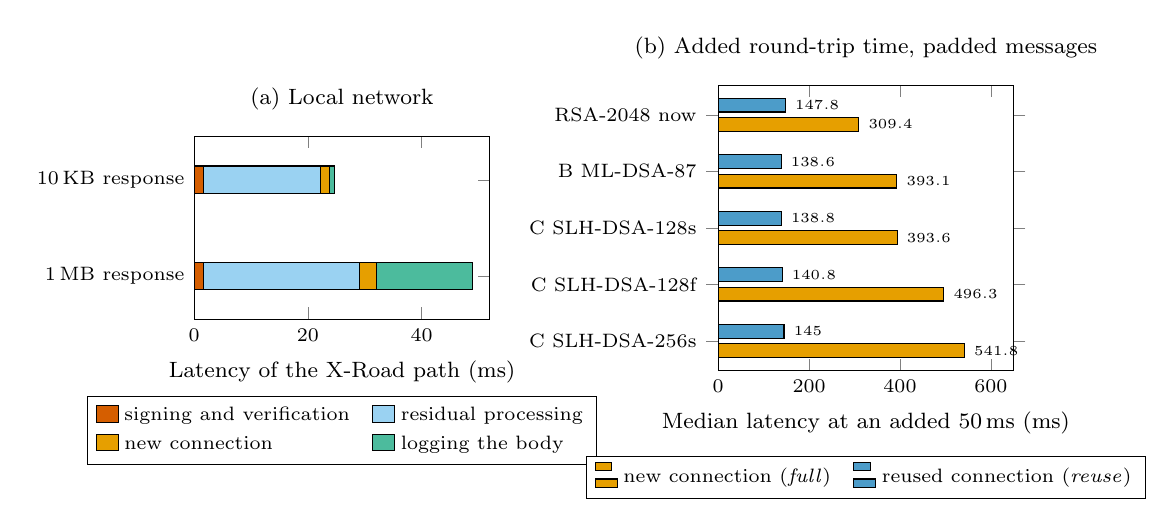
\begin{tikzpicture}
\begin{axis}[name=pa, xbar stacked, width=0.44\textwidth, height=3.9cm, bar width=10pt,
  xmin=0, xmax=52, ytick=data, symbolic y coords={1\,MB response,10\,KB response},
  enlarge y limits=0.45, xlabel={Latency of the X-Road path (ms)},
  title={(a) Local network}, title style={font=\footnotesize},
  tick label style={font=\scriptsize}, label style={font=\footnotesize},
  legend style={font=\scriptsize, at={(0.5,-0.42)}, anchor=north, legend columns=2,
    /tikz/every even column/.append style={column sep=0.6em}}, legend cell align=left]
\addplot[fill=okVermillion, draw=black] coordinates {(1.7,10\,KB response) (1.7,1\,MB response)};
\addlegendentry{signing and verification}
\addplot[fill=okSky!60, draw=black] coordinates {(20.5,10\,KB response) (27.4,1\,MB response)};
\addlegendentry{residual processing}
\addplot[fill=okOrange, draw=black] coordinates {(1.6,10\,KB response) (2.9,1\,MB response)};
\addlegendentry{new connection}
\addplot[fill=okGreen!70, draw=black] coordinates {(0.9,10\,KB response) (17.0,1\,MB response)};
\addlegendentry{logging the body}
\end{axis}
\begin{axis}[at={(pa.east)}, anchor=west, xshift=2.9cm, xbar, width=0.44\textwidth, height=5.2cm,
  bar width=5pt, xmin=0, xmax=650, ytick=data,
  symbolic y coords={C SLH-DSA-256s,C SLH-DSA-128f,C SLH-DSA-128s,B ML-DSA-87,RSA-2048 now},
  enlarge y limits=0.13, xlabel={Median latency at an added 50\,ms (ms)},
  title={(b) Added round-trip time, padded messages}, title style={font=\footnotesize},
  tick label style={font=\scriptsize}, label style={font=\footnotesize},
  legend style={font=\scriptsize, at={(0.5,-0.3)}, anchor=north, legend columns=2,
    /tikz/every even column/.append style={column sep=0.6em}}, legend cell align=left,
  nodes near coords, nodes near coords style={font=\tiny}, point meta=x]
\addplot[fill=okOrange, draw=black] coordinates {(309.4,RSA-2048 now) (393.1,B ML-DSA-87) (393.6,C SLH-DSA-128s)
  (496.3,C SLH-DSA-128f) (541.8,C SLH-DSA-256s)};
\addlegendentry{new connection (\emph{full})}
\addplot[fill=okBlue!70, draw=black] coordinates {(147.8,RSA-2048 now) (138.6,B ML-DSA-87) (138.8,C SLH-DSA-128s)
  (140.8,C SLH-DSA-128f) (145.0,C SLH-DSA-256s)};
\addlegendentry{reused connection (\emph{reuse})}
\end{axis}
\end{tikzpicture}
\caption{\newtext{Where the time of an exchange goes, development laptop, one client. (a) The X-Road
path (\emph{full} $-$ \emph{direct}, \newtext{Figure~\ref{fig:division}}) split into signing and verification
(benchmark, Section~\ref{sec:rq3}), \newtext{the residual processing of the Security Server (the remainder of the path minus the benchmark times, obtained by subtraction)}, opening a new connection (\emph{full} $-$ \emph{reuse}) and logging the body
(\emph{full} $-$ \emph{nobody}); synchronous time-stamping, not in the default, would add another
62--68\,ms. (b) Median latency at an added round-trip time of 50\,ms for messages padded to the size
of the present messages and of post-quantum messages in scenarios B and C (one grid,
\newtext{Section~\ref{sec:rq3}}); the post-quantum signing and verification would change it by 0.2 to
6.4\,ms.}}
\label{fig:summary}
\end{figure*}

\subsection{What the results mean for the proposed changes}\label{sec:pq}

The proposals discussed in the introduction affect different mechanisms, and the measurements put
them in different positions.

\newtext{Post-quantum signatures change signing and verification, which are paid on every message
and run on the CPU of the Security Servers. In the stage breakdown this work cannot be separated from
the other work of the same stages, but measured on its own (Section~\ref{sec:rq3}) it changes the
computation of an exchange by about a millisecond with the lattice schemes, less than the spread
between repetitions and less than the architectural costs on the local network; only the composites
with RSA-3072 and RSA-4096 and SLH-DSA in the CA add 1.6 to 9.3\,ms\newtext{, and on a CPU as slow
as that of the three machines up to about 19\,ms, comparable with the remainder of the path
(Section~\ref{sec:rq3})}. The size matters more, and it is
decided less by the members than by the infrastructure: every message carries the signing
certificate and the OCSP responses, so a change of the CA and the OCSP responder enlarges every
message, and it accounts for about three quarters of the growth (\newtext{Section~\ref{sec:rq3}}). The step at
the initial window is the one known from post-quantum TLS
handshakes~\cite{sikeridis2020,westerbaan2021,chou2026}; in X-Road it is paid on every message on a
new connection rather than once per handshake. With the default connection policy and distance
between the Security Servers messages of this size need up to two additional round trips each with
ML-DSA, one or two as soon as the CA and the OCSP responder migrate, and up to five with SLH-DSA in the CA, and none with reused connections. Keeping SLH-DSA in
the CA rather than in the member keys agrees with the placement found practical for TLS
hierarchies~\cite{delgado2026}.} The TLS handshake between the Security
Servers, which post-quantum algorithms would also enlarge~\cite{bakhtina2026pqc}, was resumed from a
session ticket without exchanging certificates in every captured message, so larger certificates would
mainly affect new sessions rather than every message. \newtext{Between the Security Servers
X-Road~7.8.3 uses TLS~1.2 only~\cite{xroadsrc}, while post-quantum key exchange and authentication
are studied and standardised for TLS~1.3~\cite{paquin2020,sikeridis2020}, so a post-quantum channel
would first require X-Road to move to TLS~1.3. Full handshakes are not rare either: a consumer that
exchanges messages with many providers, or whose session ticket has expired, sets up new sessions,
and with post-quantum certificates each of them would carry larger certificate chains that can add
round trips of their own~\cite{sikeridis2020}. This cost is not estimated here.}

A decentralised PKI changes how certificates are checked~\cite{bakhtina2023ares}. In the present
system status checking was not part of the request path: the Security Server took the status from
its cache, and requests to the OCSP responder appeared only when a background refresh fell into a
run. Any per-request
presentation of credentials would therefore be a new cost in the request path rather than a
replacement of an existing one.

Threshold signatures change signing~\cite{bakhtina2026ijis}. Their reported round trips of 191 to
272\,ms for small threshold groups, against 32\,ms with a single software token, are several times the
whole cost of X-Road measured here with one client on the local network, and of the same order as the
effect of the connection policy with an added round-trip time of 50\,ms.

\subsection{The connection policy}

Among the configurations compared, the largest effect is the decision to open a new connection for
every message. On the local network it costs about 2\,ms and 6.2\,KB per exchange (3.3\,KB towards the provider
and 2.9\,KB back),
which is why it is easy to overlook. With an added round-trip time every message waits for several
additional round trips, and at 50\,ms reusing connections saves 54\,\% of the latency for a 10\,KB
response and 72\,\% for a 1\,MB response, and almost doubles the throughput with 16 clients. This
agrees with the observation that the cost of TLS depends mostly on whether connections are
reused~\cite{naylor2014}. Connection reuse is off by default~\cite{xroadsyspar}, so its benefit grows
with the distance between the Security Servers of the communicating organisations. It is not free of
side effects either: in the measurements, single requests over reused connections failed, consistent
with a pooled connection that had already been closed by the other side. \newtext{The documentation
of X-Road also gives a reason for the default: without pooled connections every connection is closed
after one message, which is recommended for Security Servers behind a load balancer so that it can
distribute the traffic evenly~\cite{xroadsyspar,xroadxlb}. Whether the failures observed with reused
connections would also occur in production, and whether their rate, \newtext{up to} two requests in 10\,000
under load, is acceptable for the services that use X-Road, was not examined. Enabling reuse is
therefore a trade-off for the operators rather than a free improvement.}

The connection policy also decides how much larger post-quantum messages cost. \newtext{With reused
connections the TCP window is already open, and none of the schemes in Table~\ref{tab:pq} needed an
additional round trip. With a new connection for every message they need up to two additional round
trips with ML-DSA, Falcon and the composites and up to five with SLH-DSA in the CA; at an added
50\,ms one or two round trips are 50 to 100\,ms per message, against the 153\,ms that reusing
connections already saves for a 10\,KB response (\newtext{Section~\ref{sec:rtt}}).}

\subsection{Comparison with earlier measurements}

{\color{blue}Table~\ref{tab:related} compares the results with the earlier work on X-Road and on \newtext{post-quantum signatures; the
comparisons with TLS connection reuse and post-quantum certificate chains in TLS are made above}.\par}

\begin{table*}[!b]
\centering\small
\caption{\newtext{Earlier work compared with the results of this study, where the comparison is not
made in the text.}}
\label{tab:related}
\color{blue}
\begin{tabular}{@{}p{0.15\textwidth}p{0.38\textwidth}p{0.41\textwidth}@{}}
\toprule
Work & Setting and result & This study \\
\midrule
Ansper et al.~\cite{ansper2013} & Design of batched time-stamping, analytical estimate; the
implementation not benchmarked & About two requests to the time-stamping service per 1200 messages;
the synchronous policy adds 89--92\,ms and lowers the throughput ceiling to 37--47\,\% \\
\addlinespace
Taklai~\cite{taklai2020} & Security Server in front of a registry service, 10--30 clients; database
time dominates; the path through the Security Server faster than the direct one at 20 and 30
clients & Spread under load 15--41\,\% on three machines, too large to compare the configurations;
only the ceilings and \emph{synctsa} are reported \\
\addlinespace
Bakhtina et al.~\cite{bakhtina2026ijis} & X-Road 7.7.0, all components on one laptop, mean of 1000
requests: 32\,ms with a software token, 191--272\,ms with threshold signatures & 25--30\,ms with one
client in three environments; \newtext{throughput 1.4--1.8 times higher on three machines than on one} \\
\addlinespace
Snetkov and Vakarjuk~\cite{snetkov2023} & Post-quantum signatures in UXP: a Dilithium5 signature
takes 4595 bytes against 256 for RSA-2048 (ML-DSA-87: 4627); no timing & \newtext{Two such signatures would
add about 8.7\,KB to an exchange of about 40\,KB; with the certificates and OCSP responses in every
message, ML-DSA adds 4.6--41\,KB and 0--2 round trips on a new connection (Table~\ref{tab:pq})} \\
\addlinespace
Müller and Oupický~\cite{mueller2024} & Post-quantum and hybrid XML signatures in Apache Santuario
and BouncyCastle; signing and verification time and document size, without certificate chains or
network & The same libraries; per exchange the post-quantum signatures change the computation by
about 1\,ms, while their size costs round trips on new connections \\
\addlinespace
Vakarjuk et al.~\cite{vakarjuk2024} & Obstacles to post-quantum migration in the Estonian
e-government systems; signatures for X-Road should be short; no measurement & Signatures of the
infrastructure make up about three quarters of the growth of a message; the size costs round trips
only on new connections \\
\addlinespace
Abbasi et al.~\cite{abbasi2025}, Rahul et al.~\cite{rahul2026}, Demir et al.~\cite{demir2026} &
Post-quantum (m)TLS~1.3: operations below 1\,ms, less than 5\,\% added latency on servers, about
3\,\% of the CPU time in cryptography; the cost lies in the handshake size & The same order in
X-Road: the signatures of an exchange take less than a tenth of the remainder of the path, and the
size enlarges every message, not only the handshake \\
\bottomrule
\end{tabular}
\end{table*}


\newtext{The single-host figure of~\cite{bakhtina2026ijis} was presented as a lower bound because
there was no network between the servers. For one client on a local network it is representative,
since the network cost is offset by the provider having a CPU of its own, but not for throughput or
for Security Servers that are farther apart, where the connection policy dominates. That the path
through the Security Server appeared faster than the direct one under load~\cite{taklai2020}
suggests that the variation of the environment was comparable to the effect being measured, as the
spread under load was here, while with one client and with an added round-trip time it mostly stayed
within a few per cent.}

The warm-up needed was much longer than the earlier work suggests. The closest measurement reports
means over 1000 requests without describing a warm-up~\cite{bakhtina2026ijis}, while here the latency did not settle
within the first thousand requests and the first run after a restart stayed slower even after 4000, in line with
the advice to measure Java systems only in the steady state~\cite{georges2007}. Short measurements of
X-Road may therefore overestimate its latency and vary more between runs.

\subsection{Absolute values and differences}

The absolute values depend on the hardware: the same grid gave 24.8\,ms on the development laptop and
28.3\,ms on the three machines for a 10\,KB response, and the CPU-bound costs, logging a large body
and synchronous time-stamping, differed by up to a factor of two. The differences between
configurations kept their sign and order in every environment, and the effect of the connection
policy on the local network was about the same (1.6--2.0\,ms at 10\,KB). The power mode of the CPU had an
even larger effect than the choice of machine. Measurements of X-Road on general-purpose hardware
should therefore report the CPU and its power mode together with the results.

\subsection{\newtext{Threats to validity}}\label{sec:threats}

Several properties of the testbed shift the absolute values. The machines are laptops rather than
servers, and the development laptop adds the overhead of WSL~2 on Windows. The time-stamping service
of the test CA is a replacement, and the images of the test CA and the load generator were not pinned
to a version. The test CA, OCSP
responder and time-stamping service run next to the Security Servers, whereas in production they are
external services with their own latency, so the figures for status checking and synchronous
time-stamping are optimistic. All intervals of the background mechanisms are left at their defaults,
while a production deployment may use longer ones: for the Estonian instance of 2017 a master's
thesis documents a global configuration validity of six hours and an OCSP freshness of eight
hours~\cite{mironova2017}, so background costs per message would be even lower there than in the
testbed.

Other properties change the shares and the spread rather than the absolute values. The echo service
has no processing time of its own, which raises the relative share of the trust mechanisms compared
with a real service. Under load the spread between repetitions is larger, so there the stable
throughput and the results of synchronous time-stamping are reported together with the spread and
the errors, and small differences between the other configurations are not assigned to individual
mechanisms. The added round-trip time is emulated:
it has no cross traffic and no losses, and it is applied inside the hosts of the Security
Servers\newtext{, which is checked by applying it to incoming instead of outgoing packets
(Section~\ref{sec:delay})}\newtext{; this did not change the slopes (Section~\ref{sec:rtt})}.
\newtext{The response bodies are random bytes, so that the message log cannot compress them; real
JSON or XML messages compress well, so the cost of logging a large body is a worst case. The member
keys are in software tokens, whereas production Security Servers often keep them in hardware
security modules, where signing goes through PKCS\#11 and may take considerably longer. The cause of
the large spread of throughput under load, such as throttling of the laptop CPUs, garbage collection
of the Java virtual machine or the database, was not investigated.} \newtext{The sizes of 10\,KB and
1\,MB were chosen as a small and a large message, not from the distribution of message sizes in a real
X-Road instance, which was not available, and the workload uses one request pattern against an echo
service. Where a configuration made no difference, this means a difference below the spread between
repetitions and, for the stages, below the resolution of 1\,ms, not a cost of zero. The model of the
flights holds for the tested TCP configuration: other initial windows, congestion control algorithms,
packet loss or limited bandwidth were not examined.}

\newtext{The estimate for post-quantum signatures is not a measurement of X-Road with them. It
assumes that the computation and the round trips add up, which was not checked.} \newtext{The padded
messages reproduce the size of post-quantum messages but not where the additional bytes are: in a
real message they would be in the XML signature, the certificates and the OCSP responses rather than
in the body, and the order in which X-Road writes the parts of a message into TLS records could shift
the boundaries of the flights. Nor do they include the processing of the larger structures inside
X-Road, such as parsing larger certificates and OCSP responses, canonicalising XML with longer
base64 values and logging larger signatures, or the way post-quantum signatures would eventually be
integrated into X-Road, for example as a composite or as two separate signatures, which could change
both the size and the number of operations.} \newtext{The} \newtext{estimated} \newtext{round trips depend on the TCP settings of the testbed, the initial window of 10 segments and the
receive window of the provider, which the operating system adjusts itself, so the numbers of flights
hold for this configuration; a shrinking message, as with ECDSA in scenario B, was not checked, since
padding can only enlarge it. \newtext{The model was corrected twice where it disagreed with the
grids, each time from the traffic captures, and after the last correction it was compared only with
the points that had been measured already, not with new ones. For a message within about a segment
of the boundary of a flight the estimate can therefore be off by one round trip.} \newtext{The grids of the check
ran on the development laptop, whose latency without added delay varied between and within the
grids; the check therefore rests on the latency at the added round-trip time, compared with the
baseline of the same grid.} The authentication certificates are assumed to use the scheme of the
members and the same CA, and the certificates of the TLS handshake are not included, since a resumed
TLS session does not exchange them. The computation is measured with the
implementations of BouncyCastle~1.84 on Java~21, the versions of X-Road~7.8.3. Java has its own
ML-DSA only from Java~24~\cite{jep497}, and an implementation of another library or of a later Java
version may take a different time~\cite{oleksiichuk2026}. The
signer of X-Road receives only a digest, while ML-DSA and SLH-DSA in their pure form sign the data
itself, so X-Road would need their pre-hash variants~\cite{fips204,fips205} or a change of this
interface; \newtext{the pre-hash variants were benchmarked only for ML-DSA, SLH-DSA-128f and three
composites, not for Falcon, and not inside the signer of X-Road}. The
composites of BouncyCastle~1.84 follow the drafts that preceded RFC~10073; their object identifiers
match it, but their signatures were not compared with its test vectors.}

Because of these factors the absolute latencies describe this testbed rather than a production
deployment. The comparisons are therefore made between configurations on the same machines and
under the same conditions, and the results are read primarily as differences between configurations
and as their change with message size, load and added round-trip time; absolute values are reported for
reference only.

\section{Conclusion}

This study measured how much the trust mechanisms of X-Road cost per message, on three laptops
connected by a switch, on one of them alone, on a faster laptop, and with a controlled round-trip time
added between the Security Servers\newtext{. Because X-Road does not support post-quantum signatures, their cost was
estimated rather than measured: the times of the signature schemes, benchmarked on their own, were
combined with what RQ1 and RQ2 showed about the path, namely how many signatures an exchange makes and
verifies and how the size of a message turns into round trips. The estimate was checked on the testbed
with messages padded to the post-quantum sizes}.

For RQ1, the X-Road path added about 28\,ms to a 10\,KB exchange with one client on these machines.
Logging the message body made no measurable difference for small messages and accounted for almost
half of the latency of a 1\,MB exchange. Opening a new connection for every message cost about 2\,ms
and 6.2\,KB per exchange on the local network. Certificate status checking and batched time-stamping
were not in the request path \newtext{in the steady state, with valid cached OCSP responses}: requests to the OCSP responder only from background refreshes and about two time-stamping
requests per 1200 messages,
while synchronous time-stamping added about 90\,ms. Signing and verification cannot be switched off;
\newtext{measured on their own, they take 1.7\,ms per exchange on the development laptop, less than
a tenth of the 22\,ms that remain of the path there once the costs that configuration can change are
removed. The division is therefore threefold: the cryptographic operations are small, the
architectural decisions that configuration can change are small on the local network but dominate
with large bodies and with distance, and the \newtext{residual processing} of the Security Server around the
cryptography is the largest part of the latency of a small message on the local network.}

For RQ2, most of the growth from a 10\,KB to a 1\,MB response came from writing the body to the
message log. Under load the Security Servers reached about 100 requests per second on three machines,
synchronous time-stamping \newtext{lowered that to 37--47\,\%}, and the spread between repetitions was too large to compare
the other configurations\newtext{; for load, the study therefore answers RQ2 only with the highest
throughput observed at 4, 16 and 32 clients and the effect of synchronous time-stamping, not with
full throughput--latency curves}.

\newtext{Also for RQ2}, one machine and three machines gave nearly the same latency and differences with one
client, while three machines reached a higher throughput. With an added round-trip time the default
connection policy made every message wait for about five round trips at 10\,KB and ten at 1\,MB,
against two with reused connections; a prediction from the handshakes alone gave three and one and
missed two waits inside TCP.

\newtext{For RQ3, post-quantum signatures, estimated from a benchmark on the Java version and the
library of X-Road and from a model of the TCP flights checked on the testbed, change the computation
of an exchange by about a millisecond with the lattice schemes, less than the architectural costs,
and by up to 9\,ms with the composites with RSA and with SLH-DSA in the CA\newtext{, which on the
slower CPU of the three machines would be up to about 19\,ms, comparable with the remainder of the
path}. Messages of their size
need no additional round trip with reused connections, but on a new connection one or two with ML-DSA
once the CA and the OCSP responder migrate, and up to five with SLH-DSA in the CA; most of this growth comes from the
signatures of the infrastructure, which every message carries.} \newtext{The computation is the
same for the pre-hash variants that the signer of X-Road, which receives only a digest, would
need.} \newtext{These figures concern the
signatures of the messages; post-quantum key exchange and certificates in the TLS handshake between
the Security Servers, which X-Road would first have to move to TLS~1.3, are not part of the
estimate.}

The results give a baseline for the present system against which post-quantum signatures, a
decentralised PKI and threshold signatures can be compared. \newtext{They also indicate that, under
the evaluated conditions and the tested TCP configuration, the latency cost of larger post-quantum
signatures comes from connection set-up and the TCP window rather than from the cryptography: with
reused connections the padded messages needed no additional round trip, while with a new connection
for every message and Security Servers far apart they cost round trips on every message.} Further work could measure post-quantum
signatures once they are available in X-Road, repeat the measurements with external certification and
time-stamping services and over a real wide-area link, and use server hardware.

\begin{thebibliography}{99}

\bibitem{mayer1995}
R.~C.~Mayer, J.~H.~Davis, F.~D.~Schoorman.
\newblock An Integrative Model of Organizational Trust.
\newblock \emph{Academy of Management Review}, 20(3):709--734, 1995.

\bibitem{grandison2000}
T.~Grandison, M.~Sloman.
\newblock A Survey of Trust in Internet Applications.
\newblock \emph{IEEE Communications Surveys \& Tutorials}, 3(4):2--16, 2000.

\bibitem{anderson2020}
R.~Anderson.
\newblock \emph{Security Engineering: A Guide to Building Dependable Distributed Systems}, 3rd ed.
\newblock Wiley, 2020.

\bibitem{bakhtina2023sac}
M.~Bakhtina, R.~Matulevi\v{c}ius, A.~Awad, P.~Kivim\"{a}ki.
\newblock On the Shift to Decentralised Identity Management in Distributed Data Exchange Systems.
\newblock In \emph{SAC '23}, pp.~864--873, ACM, 2023.
\newblock DOI: 10.1145/3555776.3577678.

\bibitem{xroadarcss}
Nordic Institute for Interoperability Solutions.
\newblock X-Road: Security Server Architecture.
\newblock \url{https://docs.x-road.global/Architecture/arc-ss_x-road_security_server_architecture.html}.
\newblock Accessed 17 September 2026.

\bibitem{ansper2013}
A.~Ansper, A.~Buldas, M.~Freudenthal, J.~Willemson.
\newblock High-Performance Qualified Digital Signatures for X-Road.
\newblock In \emph{NordSec 2013}, LNCS 8208, pp.~123--138, Springer, 2013.

\bibitem{bakhtina2026ijis}
M.~Bakhtina, J.~Kvapil, P.~\v{S}venda, R.~Matulevi\v{c}ius.
\newblock Securing Organisational Digital Identity: A Full-Lifecycle Approach to Distributed Key
Management.
\newblock \emph{International Journal of Information Security}, 25:131, 2026.
\newblock DOI: 10.1007/s10207-026-01291-5.

\bibitem{taklai2020}
E.~Taklai.
\newblock X-tee teenuste j\~{o}udlustestimine Eesti \"{a}riregistri n\"{a}itel
(Performance testing of X-Road services on the example of the Estonian Business Register).
\newblock Diploma thesis, Tallinn University of Technology, 2020.

\bibitem{xteefactsheet}
Estonian Information System Authority (RIA).
\newblock X-tee Factsheet, Estonia.
\newblock \url{https://www.x-tee.ee/factsheets/EE/}.
\newblock Figures based on data of 1 September 2026; accessed 17 September 2026.

\bibitem{bakhtina2026pqc}
M.~Bakhtina.
\newblock Migration of X-Road to Post-Quantum Cryptography.
\newblock NIIS Publication series, Nordic Institute for Interoperability Solutions, 2026.
\newblock ISBN 978-9916-9853-4-2.

\bibitem{snetkov2023}
N.~Snetkov, J.~Vakarjuk.
\newblock Integrating Post-Quantum Cryptography to UXP.
\newblock Cybernetica Research Report D-2-499, 2023.

\bibitem{vakarjuk2024}
\textcolor{blue}{J.~Vakarjuk, N.~Snetkov, P.~Laud.
\newblock Identifying Obstacles of PQC Migration in e-Estonia.
\newblock In \emph{16th International Conference on Cyber Conflict (CyCon 2024)}, pp.~63--81,
NATO CCDCOE, 2024.
\newblock DOI: 10.23919/CyCon62501.2024.10685570.}

\bibitem{bakhtina2023ares}
M.~Bakhtina, K.~L.~Leung, R.~Matulevi\v{c}ius, A.~Awad, P.~\v{S}venda.
\newblock A Decentralised Public Key Infrastructure for X-Road.
\newblock In \emph{ARES 2023}, ACM.
\newblock DOI: 10.1145/3600160.3605092.

\bibitem{coarfa2006}
\textcolor{blue}{C.~Coarfa, P.~Druschel, D.~S.~Wallach.
\newblock Performance Analysis of TLS Web Servers.
\newblock \emph{ACM Transactions on Computer Systems}, 24(1):39--69, 2006.
\newblock DOI: 10.1145/1124153.1124155.}

\bibitem{naylor2014}
D.~Naylor, A.~Finamore, I.~Leontiadis, Y.~Grunenberger, M.~Mellia, M.~Munaf\`{o},
K.~Papagiannaki, P.~Steenkiste.
\newblock The Cost of the ``S'' in HTTPS.
\newblock In \emph{CoNEXT '14}, pp.~133--140, ACM, 2014.
\newblock DOI: 10.1145/2674005.2674991.

\bibitem{paquin2020}
C.~Paquin, D.~Stebila, G.~Tamvada.
\newblock Benchmarking Post-quantum Cryptography in TLS.
\newblock In \emph{PQCrypto 2020}, LNCS vol.~12100, pp.~72--91, Springer, 2020.
\newblock Cryptology ePrint Archive 2019/1447.

\bibitem{sikeridis2020}
\textcolor{blue}{D.~Sikeridis, P.~Kampanakis, M.~Devetsikiotis.
\newblock Post-Quantum Authentication in TLS 1.3: A Performance Study.
\newblock In \emph{NDSS 2020}, Internet Society, 2020.
\newblock DOI: 10.14722/ndss.2020.24203.}

\bibitem{westerbaan2021}
\textcolor{blue}{B.~Westerbaan.
\newblock Sizing Up Post-Quantum Signatures.
\newblock Cloudflare blog, 8 November 2021.
\newblock \url{https://blog.cloudflare.com/sizing-up-post-quantum-signatures/}.}
\newblock \newtext{Accessed 19 November 2026.}

\bibitem{chou2026}
\textcolor{blue}{M.~Chou, P.~Cao.
\newblock Network Impact of Post-Quantum Certificate Chain Sizes on Time to First Byte in TLS
Deployments.
\newblock arXiv:2604.24869, 2026.}

\bibitem{kampanakis2024}
\textcolor{blue}{P.~Kampanakis, W.~Childs-Klein.
\newblock The Impact of Data-Heavy, Post-Quantum TLS 1.3 on the Time-To-Last-Byte of Real-World
Connections.
\newblock In \emph{MADWeb 2024}, Internet Society, 2024.
\newblock DOI: 10.14722/madweb.2024.23010.}

\bibitem{abbasi2025}
\newtext{M.~Abbasi, F.~Cardoso, P.~V{\'a}z, J.~Silva, P.~Martins.
\newblock A Practical Performance Benchmark of Post-Quantum Cryptography Across Heterogeneous
Computing Environments.
\newblock \emph{Cryptography}, 9(2):32, 2025.
\newblock DOI: 10.3390/cryptography9020032.}

\bibitem{rahul2026}
\newtext{Rahul, M.~K.~Hanawal, S.~G.~Kulkarni, Saravanan~V, K.~T.~Reddy.
\newblock PQC Migration: End-to-End Performance Profiling of Post Quantum Cryptographic Algorithms in
mTLS.
\newblock arXiv:2611.21206, 2026.}

\bibitem{demir2026}
\newtext{E.~D.~Demir, I.~Gorgulu, M.~C.~Onba{\c{s}}l{\i}.
\newblock Micro and Transport Layer Security Benchmarking of Post-Quantum Versus Classical
Cryptography.
\newblock \emph{IEEE Access}, 14, 2026.
\newblock DOI: 10.1109/ACCESS.2026.3682760.}

\bibitem{mueller2024}
\textcolor{blue}{J.~M{\"u}ller, J.~Oupick{\'y}.
\newblock Post-quantum XML and SAML Single Sign-On.
\newblock \emph{Proceedings on Privacy Enhancing Technologies}, 2024(4):525--543, 2024.
\newblock DOI: 10.56553/popets-2024-0128.}

\bibitem{xroadsyspar}
Nordic Institute for Interoperability Solutions.
\newblock X-Road: System Parameters (UG-SYSPAR)\newtext{, version 2.103 of 24 March 2026}.
\newblock \url{https://docs.x-road.global/Manuals/ug-syspar_x-road_v6_system_parameters.html}.
\newblock Accessed 17 September 2026.

\bibitem{kivimaki2020}
P.~Kivim\"{a}ki.
\newblock Resisting Failure.
\newblock NIIS blog, \newtext{26} November 2020.
\newblock \url{https://www.niis.org/blog/2020/11/20/resisting-failure}.
\newblock \newtext{Accessed 19 November 2026.}

\bibitem{xroadmesstransp}
\newtext{Nordic Institute for Interoperability Solutions.
\newblock X-Road: Message Transport Protocol (PR-MESSTRANSP), version 2.7.
\newblock \url{https://docs.x-road.global/Protocols/pr-messtransp_x-road_message_transport_protocol.html}.
\newblock Accessed 20 November 2026.}

\bibitem{xroadsrc}
\newtext{Nordic Institute for Interoperability Solutions.
\newblock X-Road source code, version 7.8.3.
\newblock \url{https://github.com/nordic-institute/X-Road/tree/7.8.3}.
\newblock Accessed 19 November 2026.}

\bibitem{k6}
\newtext{Grafana Labs.
\newblock Grafana k6, load testing tool.
\newblock \url{https://k6.io/}.
\newblock Accessed 19 November 2026.}

\bibitem{chrony}
\newtext{The chrony project.
\newblock chrony, an implementation of the Network Time Protocol.
\newblock \url{https://chrony-project.org/}.
\newblock Accessed 19 November 2026.}

\bibitem{hemminger2005}
S.~Hemminger.
\newblock Network Emulation with NetEm.
\newblock In \emph{linux.conf.au 2005}, Canberra, 2005.

\bibitem{nussbaum2009}
L.~Nussbaum, O.~Richard.
\newblock A Comparative Study of Network Link Emulators.
\newblock In \emph{Communications and Networking Simulation Symposium (CNS '09)}, 2009.

\bibitem{jurgelionis2011}
A.~Jurgelionis, J.-P.~Laulajainen, M.~Hirvonen, A.~I.~Wang.
\newblock An Empirical Study of NetEm Network Emulation Functionalities.
\newblock In \emph{ICCCN 2011}, IEEE, 2011.

\bibitem{georges2007}
A.~Georges, D.~Buytaert, L.~Eeckhout.
\newblock Statistically Rigorous Java Performance Evaluation.
\newblock In \emph{OOPSLA '07}, pp.~57--76, ACM, 2007.
\newblock DOI: 10.1145/1297027.1297033.

\bibitem{fips204}
National Institute of Standards and Technology.
\newblock Module-Lattice-Based Digital Signature Standard.
\newblock FIPS 204, 2024.
\newblock DOI: 10.6028/NIST.FIPS.204.

\bibitem{rfc10073}
M.~Ounsworth, J.~Gray, M.~Pala, J.~Klau{\ss}ner, S.~Fluhrer.
\newblock Composite Module-Lattice-Based Digital Signature Algorithm (ML-DSA) for Use in X.509
Public Key Infrastructure.
\newblock RFC 10073, IETF, 2026.

\bibitem{fips205}
National Institute of Standards and Technology.
\newblock Stateless Hash-Based Digital Signature Standard.
\newblock FIPS 205, 2024.
\newblock DOI: 10.6028/NIST.FIPS.205.

\bibitem{delgado2026}
\textcolor{blue}{J.~L.~Delgado Jim{\'e}nez.
\newblock Signature Placement in Post-Quantum TLS Certificate Hierarchies: An Experimental Study of
ML-DSA and SLH-DSA in TLS 1.3 Authentication.
\newblock arXiv:2604.06100, 2026.}

\bibitem{bouncycastle}
\newtext{Legion of the Bouncy Castle.
\newblock Bouncy Castle Crypto APIs for Java, version 1.84.
\newblock \url{https://www.bouncycastle.org/download/bouncy-castle-java/}.
\newblock Accessed 19 November 2026.}

\bibitem{oleksiichuk2026}
\textcolor{blue}{Yu.~Oleksiichuk.
\newblock Empirical Performance Evaluation of NIST Post-Quantum Cryptographic Algorithms ML-KEM, ML-DSA,
and SLH-DSA across JDK Versions.
\newblock \emph{Cybersecurity: Education, Science, Technique}, 1(33), 2026.
\newblock DOI: 10.28925/2663-4023.2026.33.1210.}

\bibitem{jmh}
\newtext{OpenJDK.
\newblock Java Microbenchmark Harness (JMH).
\newblock \url{https://github.com/openjdk/jmh}.
\newblock Accessed 19 November 2026.}

\bibitem{rfc9110}
\newtext{R.~Fielding, M.~Nottingham, J.~Reschke.
\newblock HTTP Semantics.
\newblock RFC 9110, IETF, 2022.}

\bibitem{mironova2017}
L.~Mironova.
\newblock X-tee platvormi kriitiliste kesksete teenuste testimine
(Testing of the critical central services of the X-Road platform).
\newblock Master's thesis, Tallinn University of Technology, 2017.

\bibitem{xroadxlb}
\newtext{Nordic Institute for Interoperability Solutions.
\newblock X-Road: External Load Balancer Installation Guide (IG-XLB), version 1.30.
\newblock \url{https://docs.x-road.global/Manuals/LoadBalancing/ig-xlb_x-road_external_load_balancer_installation_guide.html}.
\newblock Accessed 19 November 2026.}

\bibitem{jep497}
\textcolor{blue}{OpenJDK.
\newblock JEP 497: Quantum-Resistant Module-Lattice-Based Digital Signature Algorithm.
\newblock Delivered in JDK 24.
\newblock \url{https://openjdk.org/jeps/497}.}
\newblock \newtext{Accessed 19 November 2026.}

\end{thebibliography}

\end{document}
